\documentclass[arial, utf8, zavrsni]{fer}
\usepackage{booktabs}
\usepackage{algorithm,algpseudocode}
\usepackage{hyperref}
\hypersetup{
    colorlinks,
    citecolor=black,
    filecolor=black,
    linkcolor=black,
    urlcolor=black
}

\usepackage{subcaption}

\begin{document}

% Dodavanje zahvale ili prazne stranice. Ako ne želite dodati zahvalu, naredbu ostavite radi prazne stranice.
\zahvala{Zahvaljujem se mentoru, prof. Marku Subašiću na potpori i savjetima na putu kroz nepoznato. Hvala mojoj obitelji te Lei, na svoj potpori koju su mi pružili i nastavljaju pružati.}

\setcounter{tocdepth}{2} %podešava dubinu sadržaja
\tableofcontents

\chapter{Uvod}
U današnjem svijetu podataka iz dana u dan ima sve više. Međutim, iako je do podataka danas vrlo lako doći, izvući korisno znanje iz njih se može pokazati kao vrlo težak zadatak. Računalni vid je jedno od područja umjetne inteligencije koje na osnovu 2D slika i videozapisa - podataka, nastoji dobiti što više informacija, odnosno korisnog znanja. Primjene ovog područja su brojne, od autonomne vožnje i cestovne sigurnosti do primjena u zdravstvu i medicini. Jedna od metoda koja se zadnjih godina pokazala najuspješnijom su duboki neuronski modeli, matematički modeli učenja zasnovani na principu rada ljudskog mozga.

Međutim, da bi duboki modeli bili uspješni, potrebne su im velike količine označenih podataka, do kakvih je često vrlo teško doći. Kako bi se riješio taj problem, razvijena su brojna rješenja, među koje spada i polunadzirano učenje - prisutp učenju dubokih mreža gdje, uz dio označenih podataka, model koristi i određen broj neoznačenih podataka kako bi poboljšao učenje. Jedan od takvih modela je i cycleGAN, nadogradnja popularne GAN arhitekture, posebice korisne u primjenama u računalnom vidu, kad je broj označenih podataka ograničen. 

U ovom radu opisat ću osnove dubokih neuronskih mreža, s posebnim naglaskom na duboke konvolucijske modele. Predstavit ću i koncept generativnih mreža, te ću se posebno fokusirati na jednu konkretnu generativnu mrežu - cycleGAN. Predloženu arhitekturu primijenit ću za rješavanje problema semantičke segmentacije ortopanograma, što je problem koji ima brojne praktične primjene. Rezultate predložene arhitekture ću usporediti s rezultatima postojećih diskriminativnih mreža, te donijeti zaključak koji pristup je prikladniji za navedeni problem.
\chapter{Računalni vid}

Računalni vid \engl{computer vision} je grana računarske znanosti, točnije područja umjetne inteligencije, koja pokušava omogućiti računalima da interpretiraju  vizualne podatke te iz njih izvuku nove informacije. To je zasigurno jedno od trenutno najuzbudljivijih i najbrže rastućih područja umjetne inteligencije, čije primjene sežu od automatskog označavanja ljudi na slikama koje objavljujemo na Instagramu i Facebooku, sve do autonomne vožnje i primjena u medicini i znanosti. Ovo područje danas doživljava svoju renesansu, u velikom dijelu zbog pojave algoritama baziranih na dubokom učenju i napretka u računalnim resursima. No ne treba zaboraviti da je računalni vid UI-potpun problem, te da je put koji smo morali prijeći da dođemo do današnjih uspjeha bio sve osim lagan.\\ \\
U ovom poglavlju dati ću osnovu podjelu područja računalnog vida te se kratko osvrnuti na njihovu praktičnu primjenu.
\section{Podjela računalnog vida}

Područje računalnog vida obuhvaća mnoga i raznolika područja. Analiza pokreta u video snimkama, detekcija objekata, rekonstrukcija 3D scene iz 2D slike su samo neki od primjera raznovrsnosti računalnog vida. Nas zanima jedno konkretno područje - detekcija objekata u 2D slikama. Glavni zadatak tog područja je, kako mu samo ime i kaže, izvući razne informacije o položaju objekata unutar slike. Ovisno o vrsti informacije, ovo područje dalje možemo podijeliti na klasifikaciju, lokalizaciju, detekciju, semantičku segmentaciju te segmentaciju instanci.

\subsection{Klasifikacija}
Najjednostavnija varijanta detekcije objekata, klasifikacija \engl{classification}, nastoji zadanu sliku svrstati u neku od predefiniranih klasa. Na primjer, ukoliko algoritmu za klasifikaciju kao ulaz predamo sliku na kojoj se nalazi mačić koji sjedi na livadu, mogli bismo očekivati da će algoritam slici pridijeliti oznaku \textit{mačka}, iako su na slici prisutni i drugi elementi poput trave, oblaka ili sunca. Povećanjem broja klasa težina problema se povećava. 

\subsection{Lokalizacija}
Sljedeći, nešto napredniji korak je lokalizacija \engl{localization}, odnosno utvrđivanje točne lokacije \textbf{jednog} objekta na slici. Na već spomenutom primjeru s mačićem na livadi, cilj bi nam bio označiti točnu lokaciju mačića u slici, najčešće crtanjem pravokutnika oko njegove lokacije.

\subsection{Detekcija}
Detekcija \engl{detection} je u svojoj osnovi vrlo slična lokalizaciji, samo što za razliku od lokalizacije, koja utvrđuje lokaciju jednog objekta na slici, detekcija utvrđuje točnu lokaciju svih instanci objekata za slici (za koje postoje zadane klase).  Česta primjena ove vrste detekcije objekata je u autonomnoj vožnji, gdje je za upravljački softver vrlo važno da zna točnu lokaciju ostalih vozila, pješaka itd., kako bi mogao donijeti ispravnu odluku o upravljanju vozilom.

\subsection{Semantička segmentacija}
Semantička segmentacija \engl{semantic segmentation} ide korak dalje, te za svaki piksel u slici nastoji odrediti kojoj klasi pripada. Ovaj problem je znatno složeniji nego prethodna tri, jer zahtjeva značajnije razumijevanje semantike slike u odnosu na prethodne. Ova vrsta detekcije također ima primjene u sustavu za autonomnu vožnju, ali i u drugim područjima, od kojih valja istaknuti primjenu u području medicinskih slika. Ovo je pristup koji nas najviše zanima i koji ćemo pobliže istražiti u nastavku ovog rada.

\subsection{Segmentacija instanci }
Segmentacija instanci \engl{instance segmentation} je složeniji oblik semantičke segmentacije, gdje se svaki piksel u slici nastoji pridijeliti točno jednoj \textbf{instanci} određene klase. Dakle, ako na slici imamo tri mačića, pikseli kojima su oni prikazani na slici pripadat će klasi mačić, ali model će također znati razlikovati pripada li određeni piksel mačiću 1, 2 ili 3.


\begin{figure}[htb]
\centering
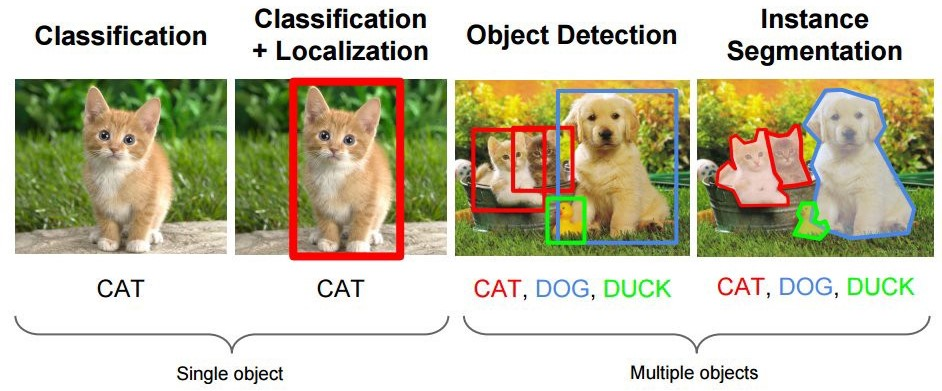
\includegraphics[width=14cm]{slike/object_detection.jpeg}
\caption{Usporedba načina detekcije \citep{objectDetectionMethodsImg}}
\label{fig:fer-logo}
\end{figure}
\textbf{}

\noindent Iako je rješavanje svih navedenih problema gotovo trivijalno za ljude, oni računalima predstavljaju velik izazov. Stoga ćemo u sljedećim poglavljima detaljnije pogledati jedan pristup koji se do sad pokazao najboljim - duboko učenje.

\chapter{Duboko učenje}
\makeatletter
\renewcommand{\ALG@name}{Algoritam}
\makeatother



Pojava i razvoj računala u drugoj polovici 20. stoljeća omogućila je automatizaciju mnogih poslova za koje su prije bili potrebni ljudi. Obrada i unos velike količine podataka, nadzor raznih proizvodnih procesa do povezivanja cijelog svijeta kroz jedinstvenu globalnu mrežu - Internet, računala su uspješno preuzela mnoge poslove za koje su prije bili nužni ljudi. No određena vrsta problema dugo je vremena izmicala pokušajima da se automatizira računalima - tzv. UI - potpuni problemi. To su problemi čija je složenost jednaka rješavanju glavnog problema umjetne inteligencije - izgradnja stroja inteligentnog poput čovjeka \citep{uilectures}. U to područje spadaju problemi poput obrade prirodnog jezika, raspoznavanja uzoraka, problemi kretanja i navigacije, te među ostalim, i područje računalnog vida. Konkretni pokušaji rješavanja ovih problema ovisili su o konkretnom problemu, te su se zasnivali na algoritamskom rješavanju problema (u području umjetne inteligencije često nazivan i simbolički pristup). Primjerice, u području računalnog vida često je bilo korištenje ručno podešenih filtera i klasifikatora za rješavanje raznih problema. No, do pravog napretka dolazi sredinom 2000-ih, pojavom dubokih neuronskih mreža, koje su uvele pravu revoluciju u područje računalnog vida.\\

\noindent U ovom poglavlju predstavit ću osnovne koncepte rada dubokih neuronskih mreža, krenuvši od opisa umjetnog neurona i jednostavne neuronske mreže, sve do složenijih dubokih modela. Također ću se osvrnuti na njihovu primjenu u području računalnog vida i problemu semantičke segmentacije, te dati primjer par najčešće korištenih arhitektura.

\section{Neuronske mreže}

Neuronsku mrežu možemo definirati kao skup međusobno povezanih procesnih jedinica (neurona) čija se funkcionalnost temelji na modelu biološkog mozga, odnosno neurona. Dakle, to je sustav koji za obradu podataka i donošenje zaključka nastoji imitirati ljudski mozak. Glavne karakteristike ovakvog pristupa, koji se često naziva i konekcionistički, su samostalno učenje na temelju predočenih podataka te mogućnost distribuirane paralelne obrade podataka. Navedene karakteristike  su u suprotnosti s algoritamskim pristupom, gdje se koraci više manje izvode slijedno, a novo znanje izvodi se pomoću predefiniranih pravila. Opis arhitekture neuronske mreže započinjemo s njenim osnovnim gradivnim elementom - neuronom. 

\subsection{Umjetni neuron}

Kako bismo bolje razumjeli model umjetnog neurona, pogledajmo prvo njegov biološki ekvivalent, kojim je i inspiriran.\\

\noindent Biološki neuroni su osnovne gradivne jedinice ljudskog mozga - prosječan ljudski mozak sadrži preko $10^{11}$ neurona, podijeljenih u preko 100 različitih vrsta. Glavni dijelovi biološkog neurona su dendriti, aksoni te tijelo (soma). 
\textbf{Dendriti} su ulazni dijelovi neurona, preko kojih neuron prima podražaje od susjednih neurona. Obrada primljenih podražaja događa se u \textbf{tijelu} neurona. U tijelu se zbrajaju sume svih podražaj primljenih preko dendrita, te se donosi odluka hoće li se neuron aktivirati ili ne. U slučaju pozitivne odluke o aktivaciji, šalje se izlazni podražaj kroz \textbf{akson} neurona.\cite{uilectures}\cite{neuroninfo}


\begin{figure}[htb]
\centering
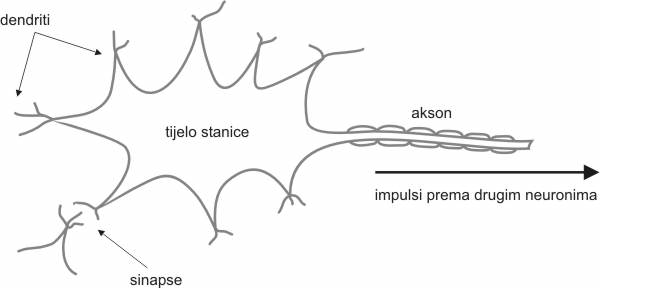
\includegraphics[width=12cm]{slike/bioloski_neuron.png}
\caption{Model biološkog neurona \citep{neuronskeMreze2008FER}}
\label{fig:fer-logo}
\end{figure}
\textbf{}
\\
Pogledamo li osnovni model umjetnog neurona, prikazan na slici 3.2, možemo primijetiti da je vrlo sličan modelu biološkog neurona. Neuron prima N numeričkih ulaza, označenih sa $\mathbf{x_{i}}$. Svakom ulazu je također pridružena i pripadajuća osjetljivost, $\mathbf{w_{i}}$, s kojom se ulaz množi prije ulaska u neuron. U neuronu se pomnoženi ulazi sumiraju, te se ukupnoj sumi dodaje pomak \engl{bias}, $\mathbf{w_{0}}$. Ovime smo definirali akumuliranu vrijednost \textit{\textbf{net}}, te ju možemo zapisati kao

\NewEnviron{myequation}{%
    \begin{equation}
    \scalebox{1.2}{$\BODY$}
    \end{equation}
    }

\begin{myequation}%
\bm{net =  (\sum\limits_{i=1}^nx_{i}   \cdot  w_{i}  )  +  w_{0}}  %
\end{myequation}


\noindent Dobivena \textit{net} vrijednost propušta se kroz \textbf{izlaznu funkciju} f \engl{activation function}, te dobivamo izlaznu vrijednost, o. \citep{uilectures}\citep{neuronskeMreze2008FER}\\

\begin{figure}[htb]
\centering
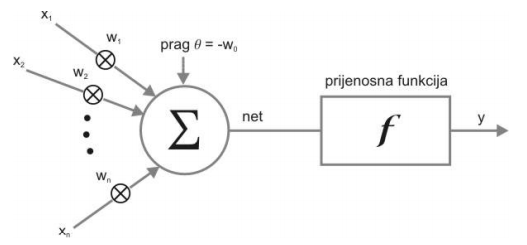
\includegraphics[width=12cm]{slike/umjetni_neuron.png}
\caption{Model umjetnog neurona \citep{neuronskeMreze2008FER}}
\label{fig:fer-logo}
\end{figure}
\textbf{}

\noindent Kako bi olakšali prikaz parametara neuronske mreže, možemo prijeći na vektorsku notaciju, gdje vektorom smatramo matricu sa točno jednim stupcem i N redaka. Onda ulaze $\mathbf{x_{i}}$ neurona možemo zapisati kao jedan vektor  $\mathbf{\overrightarrow{x} = (x_{1},x_{2}...x_{n})}$. Težine možemo prikazati vektorom $\mathbf{\overrightarrow{w} = (w_{1},w_{2}...w_{n})}$, dok pomak $\mathbf{w_{0}}$ možemo ostaviti u skalarnom obliku. Konačno, izlaz neurona o možemo zapisati kao:

\begin{myequation}%
\bm{o =  f(\overrightarrow{w}^{T} \cdot \overrightarrow{x} + b)}  %
\end{myequation}

\\
\noindent Upravo opisan model neurona se naziva TLU-perceptron \engl{Threshold logic unit}, te je prvi put predstavljen od strane McCullougha i Pittsa 1943. godine. Iako je razmjerno jednostavan, dovođenjem odgovarajućih ulaza te podešavanjem težina, pomaka i izlazne funkcije, njega već možemo koristiti za jednostavnije postupke klasifikacije i regresije. No, oni ipak imaju svoje ograničenje. To ograničenje se očituje činjenici da je \textbf{granica odluke} (skup točaka oko kojih neuron mijenja svoju odluku) TLU-perceptrona linearna, što znatno ograničava moguće primjene. Kako bismo riješili ovaj problem, prelazimo na sustave više povezanih neurona - neuronske mreže.

\subsection{Arhitektura neuronske mreže}
Neuronske mreže nisu ništa drugo osim sustavi međusobno povezanih umjetnih neurona. Svaka neuronska mreža sastoji se od više slojeva. \textbf{Sloj} je skup neurona unutar neuronske mreže koji se uvijek zajedno aktiviraju. Razlikujemo 3 vrste slojeva: ulazni sloj, skrivene slojeve te izlazni sloj.
\textbf{Ulazni sloj} služi kao ulazna točka za podatke, te uvijek postoji samo jedan.
\textbf{Izlazni sloj} je uvijek također samo jedan, te služi za izlaz iz neuronske mreže. Priroda tog izlaza ovisi o tome kako koristimo neuronsku mrežu - primjerice, koristimo li ju za klasifikaciju ulaza u N klasa, izlazni sloj može činiti N neurona, od kojih svaki kao izlaz daje vjerojatnost da ulaz pripada i-toj kasi.
\textbf{Skriveni slojevi} su glavni dio neuronske mreže, te upravo podešavanjem njihovih težina i pragova možemo neuronsku mrežu prilagoditi, odnosno naučiti nekom konkretnom problemu.
Na slici 3.3 također možemo primijetiti da svaki neuron u nekom sloju kao ulaz prima izlaze neurona iz prijašnjeg sloja. Svaka takva veza ima određenu težinu $w_{qp}$, gdje je q indeks neurona u prijašnjem sloju, a p indeks neurona u trenutnom sloju. Npr. težinu veze koja spaja neuron indeksa 1 u prijašnjem sloju te neuron indeksa 3 u trenutnom sloju mogli bismo označiti sa $w_{13}$.

\begin{figure}[htb]
\centering
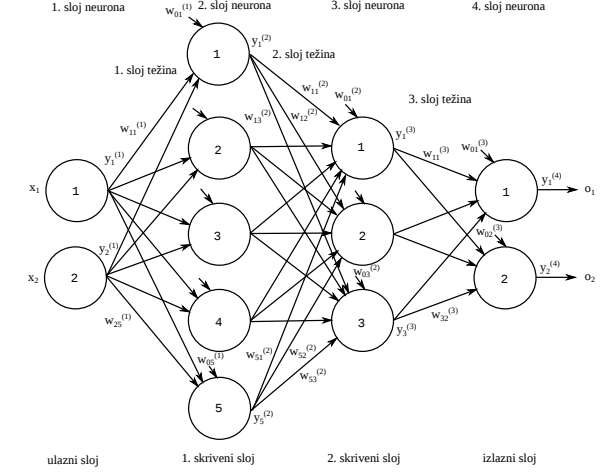
\includegraphics[width=14cm]{slike/neuronska_mreza_full.png}
\caption{Arhitektura neuronske mreže 2 x 5 x 3 x 2 \citep{umjetneNNJava}}
\label{fig:fer-logo}
\end{figure}
\textbf{}

\noindent Izlaz određenog neurona ovisi o vrijednosti izlaza neurona iz prošlog sloja, težine između trenutnog i prošlog neurona te vrijednosti praga u neuronu. Ovakve mreže, gdje izlaz neurona trenutnog sloja ovisi isključivo o izlazima neurona prethodnog sloja nazivamo \textbf{slojevitima}. Uz njih, postoje i \textbf{neslojevite} neuronske mreže, gdje izlaz neurona u nekom sloju može ovisiti o nekom neuronu više slojeva prije, ili čak o neuronu u nekom od sljedećih slojeva. Međutim, ovakve neuronske mreže nas trenutno ne zanimaju, te se u nastavku rada bavimo samo sa unaprijednim slojevitim neuronskim mrežama. \\

\noindent Sada nas još zanima kako doći do izlaza određenog sloja neuronske mreže. Kako bi olakšali zapis parametara neuronske mreže, kao i kod umjetnog neurona uvodimo vektorski zapis.
Matricu težina između i-tog i (i-1) sloja neuronske mreže možemo zapisati kao $\mathbf{W_{i}}$. Vrijednost u i-tom retku te j-tom stupcu matrice označava vrijednost težine između i-tog neurona trenutnog sloja te j-tog neurona prethodnog sloja. Ukoliko još sa $\mathbf{b_{i}}$ označimo pragove i-tog sloja neurona, izlaz i-tog sloja neuronske mreže, $h_{i}$, možemo zapisati kao:

\begin{myequation}%
\bm{\overrightarrow{h_{i}} =  f(W_{i} \cdot \overrightarrow{h_{i-1}} + b_{i})}  %
\end{myequation}

\noindent gdje je f izlazna funkcija \citep{uilectures}. Drugim riječima, izlaz svakog sloja neuronske mreže jednak je skalarnom produktu matrice težina sloja i izlaza prethodnog sloja, na koji još dodamo vektor pragova trenutnog sloja. Nad dobivenim vektorom primijenimo izlaznu funkciju, te smo dobili izlazni vektor sloja, u kojem i-ti stupac odgovara izlazu i-tog neurona u sloju. Ukoliko se radi o prvom skrivenom sloju, vektor $h_{i-1}$ je ustvari samo ulazni vektor. Vidimo da, kako bi u potpunosti definirali našu mrežu, potreban nam je vektor težina, vektor pragova i prijenosna funkcija za svaki od slojeva. Modifikacijom nekog ili svih parametara možemo promijeniti izlaz naše mreže. Upravo modifikacija navedenih parametara je jedan od ključnih dijelova u procesu učenja odnosno treniranja mreže, detaljnije obrađenog u sljedećem potpoglavlju.\\

\noindent Zadnja stvar koju je bitno napomenuti je odabir odgovarajuće prijenosne funkcije. Ako želimo da naša mreža bude ekspresivnija od običnog neurona, odnosno ako želimo modelirati i nelinearne odnose, nužno je koristiti nelinearnu prijenosnu funkciju. To je rezultat činjenice da je linearna kombinacija linearnih kombinacija također linearna kombinacija. Odnosno, ako primijenimo linearnu prijenosnu funkciju na izlaz sloja neuronske mreže, koji je i sam linearna kombinacija težina i ulaza, kao rezultat možemo dobiti samo novu linearnu kombinaciju. Najčešće korištene prijenosne funkcije uključuju sigmoidu, tangens hiperbolni, softmax i reLU, od kojih je posljednja posebice korisna prilikom treniranja dubokih modela.\citep{uilectures} 



\noindent 


\subsection{Učenje neuronskih mreža}
Učenje neuronskih mreža svodi se na mijenjanje jakosti veza između neurona - dakle na podešavanje vrijednosti pragova i težina neurona unutar mreže. Te parametre prilagođavamo kroz iterativan postupak predočavanja ulaznih primjera, najčešće u kombinaciji s očekivanim izlazom - treniranje. Stoga možemo zaključiti da je znanje o izlazu kao funkciji izlaza unutar neuronske mreže pohranjeno implicitno, kroz pragove i težine između neurona. To rezultira time da neuronske mreže najčešće funkcioniraju po principu crne kutije - za dani ulaz, vraćaju odgovarajući izlaz, međutim način na koji je neuronska mreža došla do tog izlaza je teško opisati. Takav način pohrane znanja o mapiranju ulaza na izlaze u suprotnosti je algoritamskim pristupom, gdje točno možemo opisati svaki korak pomoću kojeg smo došli do izlaza.\citep{neuronskeMreze2008FER} \\

\noindent Prije nego detaljnije opišemo postupak učenja, napomenimo da najčešće razlikujemo 3 vrste učenja. Prva, najčešće korištena metoda u svijetu dubokog učenja, je \textbf{nadzirano} \engl{supervised} učenje. Glavna karakterisika ove metode je da modelu, u ovom slučaju neuronskoj mreži, dajemo parove (ulaz, izlaz). Sustav zatim pokušava konstruirati funkciju koja će što točnije moći preslikati dani ulaz na očekivani izlaz. Druga metoda je \textbf{nenadzirano} \engl{unsupervised} učenje. U ovoj metodi modelu dajemo samo određen broj ulaza, bez pripadajućih izlaza, i modelu prepuštamo da pronađe pravilnost u podacima. Ova metoda se može primijeniti u kombinaciji sa nadziranim učenjem. Baš tu kombinaciju ćemo pobliže istražiti u nastavku ovog rada. Treća i ujedino posljednja vrsta učenja je \textbf{podržano} \engl{reinforcement} učenje. Glavni cilj ovog načina učenja je doći do niza koraka, odnosno strategije, koja rješava neki problem. 
U nastavku ćemo pogledati primjer nadziranog učenja neuronskih mreža uz pomoć jednog od najčešće korištenih algoritama - \textbf{algoritma propagacije pogreške unazad} \engl{error backpropagation}.

Kako bi objasnili algoritam, potrebno je uvesti još par pojmova. Prvi je pojam \textbf{funkcije pogreške} \engl{loss function}, često nazivane i funkcija gubitka. Već smo spomenuli da se, u svojoj osnovi, treniranje neuronskih mreža svodi na predočavanje ulaznih primjera te usporedbom dobivenog izlaza s očekivanim izlazom. Na temelju razlike između očekivanog i dobivenog izlaza modificiraju se parametri mreže. Međutim, ostaje pitanje kako točno kvantificirati razliku između ta dva izlaza? Za to nam služe funkcije gubitka. To su funkcije koje na osnovu očekivanog i dobivenog izlaza računaju jedinstvenu numeričku vrijednost pogreške. Očito, model je bolji što je vrijednost funkcije pogreške manja, stoga se učenje modela u praktičnoj primjeni zasniva na minimizaciji funkcije pogreške. U teoriji, model u kojem je svaki dobiveni izlaz jednak svakom očekivanom izlazu bi imao vrijednost funkcije pogreške jednaku 0.

Jedna od češće korištenih funkcija gubitka je (polovična) suma srednjih kvadratnih odstupanja \engl{Mean Squared Error, MSE}, koju definiramo kao:

\begin{myequation}%
\bm{MSE = \frac{1}{2N} \sum\limits_{s=1}^N \sum\limits_{i=1}^{ N_{0} }  {( t_{s,i} -  o_{s,i})} }^{2}   %
\end{myequation}

\noindent pri čemu $s$ označava redni broj para (očekivani izlaz, dobiveni izlaz), $N$ broj takvih parova, $N_{0}$ dimenziju izlaza, $t$ očekivani izlaz i $o$ dobiveni izlaz. Kvadrat u izrazu služi kako bi osigurali da će dobivena vrijednost uvije biti pozitivna, neovisno o tome je li očekivani izlaz manji ili veći od dobivenog.\\

\noindent Prisjetimo se na trenutak matematičke analize i pojma gradijenta funkcije - vektora nastalog parcijalnom derivacijom funkcije po svim njenim varijablama. On ima korisno svojstvo - pokazuje nam smjer najbržeg rasta funkcije. Jednom kada smo izračunali gradijent funkcije, možemo ga iskoristiti za minimizaciju funkcije korištenjem \textbf{tehnike gradijentnog spusta} \engl{gradient descent}. Tehnika se sastoji od malih modifikacija svake varijable funkcije u smjeru suprotnom od onog u kojem pokazuje gradijent. Ova tehnika nam garantira eventualni dolazak u neki od lokalnih minimuma funkcije. \citep{deeplearningbook}
Ova ideja se sad lako može primijeniti na funkciju gubitka neuronske mreže - funkcija gubitka je funkcija čiju vrijednost želimo minimizirati, a parametri koje prilagođavamo su upravo parametri neuronske mreže - težine i pragovi. To je upravo osnovna ideja algoritma propagacije pogreške unazad, čiju točnu definiciju dajem u nastavku. Algoritam je preuzet iz \citep{umjetneNNJava}, te pretpostavlja da je korištena sigmoidalna prijenosna funkcija:




\begin{algorithm}
  \caption{Algoritam propagacije pogreške unazad}


  
  \begin{algorithmic}
    \Statex
      1. Sve težine neuronske mreže postavi na slučajne vrijednosti
      2. \While{ uvjet zaustavljanja nije zadovoljen}:
      \Repeat
      \For{svaki uzorak $s$ iz skupa za učenje}
            \State 1. Postavi podatak $\bm{x}$ na ulaz mreže
            \State 2. Izračunaj izlaze neurona svih slojeva, od prvog prema posljednjem
            \State \hspace{1em}(izlaz posljednjeg sloja označimo sa $(o_{S,1}, ... o_{S,N_{0}})$
            \State 3. Odredi pogrešku svakog od neurona izlaznog sloja
            \State \hspace{1em} S $\delta ^{k}_{i}$ označimo pogrešku i-tog sloja te ju računamo prema izrazu:
            \State \hspace{1em} $\bm{\delta ^{K}_{i}  = o_{s,i} \cdot (1-o_{s,i}) \cdot (t_{s,i}-o_{s,i})}$, gdje je
            \State \hspace{1em} $(t_{s,i}-o_{s,i})$ - odstupanje između dobivenog i očekivanog izlaza, a
            \State \hspace{1em} $o_{s,i} \cdot (1-o_{s,i})$ - derivacija prijenosne funkcije neurona (sigmoida)
            
            \State 4. Vraćaj se sloj po sloj prema početku mreže i za svaki neuron i
            \State \hspace{1em} u sloju k računaj pogrešku prema izrazu:
            \State \hspace{1em} $\bm{\delta ^{k}_{i}  = y^{k}_{i} \cdot (1-y^{k}_{i}) \cdot   \sum\limits_{d \epsilon Downstream}^{} w_{i,d} \cdot \delta ^{k+1}_{d}}$
            \State 5. Napravi korekciju svih težina. Težinu $w^{k}_{i,j}$ korigiraj prema izrazu
            \State \hspace{1em} $\bm{w^{k}_{i,j}  \leftarrow w^{k}_{i,j} +  \eta \cdot y^{k}_{i} \cdot  \delta^{k+1}_{d}}$
            \State \hspace{1em} gdje $\eta$ predstavlja stopu učenja modela
        \EndFor
      \EndWhile
  \end{algorithmic}
\end{algorithm}

\subsection{Regularizacija i optimizacija}

Sada kada znamo osnove arhitekture i treniranja umjetnih neuronskih mreža, osvrnimo se na još dva pojma važna za izgradnju kvalitetnog modela - regularizacija i optimizacija.\\

\noindent \textbf{Regularizacija} je tehnika korištena prilikom treniranja modela koja kao cilj ima smanjiti pogrešku generalizacije modela, odnosno smanjiti prenaučenost \engl{overfitting}, ali pritom ne utjecati na pogrešku prilikom treniranja.\citep{deeplearningbook}. Regularizacija postaje sve važnija kako idemo prema dubokim, složenijim modelima, jer povećanjem složenosti modela njegova tendencija prenaučenosti raste. Najčešće korištene tehnike su augmentacija podataka te L1 i L2 regularizacija. 

\textbf{Augmentacija podataka} \engl{data augmentation} je jednostavan, ali vrlo moćan oblik regularizacije. Njegova osnovna ideja je kroz razne vrste manipulacija na umjetan način povećati broj uzoraka korištenih za treniranje. Povećanje broja uzoraka kao direktnu posljedicu ima bolju generalizaciju modela. Konkretan način augmentacije podataka ovisi o podacima koje koristimo, no primjerice ako koristimo 2D slike kao ulaz, augmentacija može uključivati razne manipulacije poput invertiranja slika, slučajnog obrezivanja dijelova slika ili dodavanja šuma.

Osnovna ideja \textbf{L1 i L2 regularizacija} je modifikacija funkcije gubitka tako da joj se doda određena dodatna vrijednost, koja ima cilj penalizirati prenaučeni model. Bez ulaženja u detalje, bez te dodatne vrijednosti model bi težio savršenoj prilagodbi podacima za treniranje, te bi loše generalizirao. Dodavanjem tog penala model "odmičemo" od pozicije u kojoj je savršeno prilagođen podacima za treniranje prema poziciji u kojoj će bolje generalizirati. Glavna razlika između L1 i L2 regularizacije je u načinu izračuna vrijednosti spomenutog penala. Konkretno, izraz za L1 je:

\begin{myequation}%
\bm{\sum\limits_{j=1}^N |w_{j}| }   %
\end{myequation}

Vidimo da se penal izračunava kao suma absolutnih vrijednosti težina mreže.  S druge strane L2 regularizaciju definiramo kao:

\begin{myequation}%
\bm{\sum\limits_{j=1}^N (w_{j})^2 }   %
\end{myequation}

Penal se izračunava kao suma kvadrata težina mreže. Konačni izraz za funkciju pogreške E prilikom korištenja L1 ili L2 regularizacije je onda:

\begin{myequation}%
\bm{E_{reg} = E_{orig} + \lambda(L) }   %
\end{myequation}

gdje je $\lambda$ parametar pomoću kojeg možemo modificirati jakost utjecaja regularizacije, a L korištena L1 ili L2 regularizacija.\citep{optimizationAndRegularization}

\noindent \textbf{Optimizacija} u kontekstu učenja neuronskih mreža najčešće podrazumijeva optimizaciju gradijentnog spusta, ključnog dijela učenja.

Jedan pristup optimizaciji gradijentnog spusta je kroz varijaciju količine podataka korištene u izračunu gradijenta funkcije pogreške. Osnovna varijanta gradijentnog spusta računa gradijent te provodi optimizaciju parametara na osnovu cijelog skupa podataka za treniranje. Ovo kao posljedicu može imati unošenje redundancije, jer će se gradijenti za slične ulazne primjere računati nekoliko puta prije ažuriranja parametara. \textbf{Stohastički gradijentni spust} provodi izračun gradijenta nakon svakog ulaznog primjera. To kao posljedicu ima ubrzanje konvergencije prema lokalnom minimumu, no također rezultira većom fluktuacijom vrijednosti funkcije pogreške.
Kombinacija ova dva pristupa je \textbf{gradijentni spust nad podskupu podataka} \engl{mini-batch gradient descent}. Ovaj pristup provodi izračun gradijenta i ažuriranje parametara modela nakon svakog podskupa svih podataka za učenje. Kako veličinu tog podskupa možemo lako mijenjati, ovo nam omogućava laku kontrolu gradijentnog spusta ovisno o konkretnom problemu koji rješavamo. \citep{gradientOptimizationAlgorithms}

Druge metode optimizaciji su znatno složenije, te uključuju metode poput Momentuma, AdaGrada, AdaDelte, i drugih. Jedan od najčešće korištenih je \textbf{Adam} \engl{Adaptive Moment Estimation}, koji ćemo ovdje ukratko opisati. Kao što smo vidjeli u Algoritmu 1, algoritam propagacije pogreške unazad, zasnivan na tehnici gradijentnog spusta, prilikom korekcije težina koristi parametar $\eta$ - stopa učenja. On određuje u kojoj mjeri će se parametri modela promijeniti - što je $\eta$ veći, to je promjena veća te model brže konvergira prema minimumu. Klasična tehnika gradijentnog spusta, pa čak i stohastičkog gradijentnog spusta koristi samo jedan $\eta$ za sve težine u modelu, te je on konstantan tijekom cijelog učenja modela. Adam, te algoritmi na kojima se on zasniva (AdaGrad i RMSProp) računa zaseban $\eta$ za svaki parametar mreže. Za računanje vrijednosti $\eta$, Adam koristi prosjek momenta prvog reda gradijenta (prosjek), ali i prosjek moment drugog reda (varijanca). \citep{AdamMachineLearningMastery} U praksi, Adam se pokazao najboljim, te se preporučuje njegova primjena. \citep{gradientOptimizationAlgorithms}

\section{Duboko učenje}
Duboko učenje, usprkos svom pomalo misterioznom i intrigantnom nazivu, zapravo nije ništa drugo već primjena dubokih neuronskih mreža na razne vrste problema. Pod pojmom \textbf{duboke neuronske mreže} najčešće podrazumijevamo bilo koju unaprijednu neuronsku s većim brojem skrivenih slojeva. Iako ne postoji točna definicija koliko slojeva neuronska mreža mora imati kako bismo ju smatrali dubokom, često se uzima uvjet od 3 ili više (skrivenih) slojeva. \citep{IBMDeepLearning}

Iako ideja dodavanja većeg broja slojeva u neuronske mreže nije ni u kojem smislu nova (prve "duboke" neuronske mreže pojavljuju se već 1990-ih godina), glavna prepreka koja je dugo kočila razvoj ovog područja je bio nedostatak adekvatnog hardvera. Razvojem adekvatnog hardvera u drugoj polovici 2000-ih te u 2010-im godinama omogućio je adekvatne resurse potrebne za treniranje i rad dubokih neuronskih mreža. Odjednom je bilo moguće trenirati dublje modele nego prije, te za treniranje koristiti skupove podataka nekoliko redova veličine iznad dotadašnjih, što je rezultiralo puno boljim rezultatima. Sve ovo je kao posljedicu imalo pravu renesansu u području dubokih neuronskih mreža, koje je ubrzo postalo najpopularnije i najbrže rastuće područje strojnog učenja. \citep{deeplearningbook}

Duboko učenje danas ostvaruje odlične rezultate u brojnim područjima primjene. Primjerice, desetak godina prije navedenih napredaka u dubokom učenju, područje raspoznavanja govora je stagniralo. Primjena metoda dubokog učenja rezultirala je u znatnom smanjenju pogrešaka modela, u nekim slučajevima i preko 50\%. Duboke mreže također postižu sjajne rezultate u području računalnog vida, primjerice u poljima semantičke segmentacije ili klasifikacije.

U nastavku ćemo se fokusirati na primjenu dubokog učenja na računalni vid, specifičnije na semantičku segmentaciju. Razmotrit ćemo jednu posebnu vrstu dubokih neuronskih mreža posebno prikladnih za ovaj problem - duboke konvolucijske mreže.


\subsection{Konvolucijske neuronske mreže}
Naša motivacija za uvođenje konvolucijskih neuronskih mreži je rješavanje problema iz domene računalnog vida. Glavni izvor podataka u tom području je naravno 2D slika. Ako želimo primijeniti duboko učenje na problem iz domene računalnog vida, moramo pronaći način kako 2D slike predati kao ulaz u model. Jedan naivan pristup bi mogao biti pretvoriti cijelu sliku u niz piksela, te svaki piksel dovesti kao jedan ulaz u mrežu. Zasigurno, mreža s takvim ulazima na raspolaganju ima sve podatke koji joj ikad mogu trebati! No uzmemo li u obzir da prosječna slika dimenzija 1980x1080 ima preko 2 milijuna piksela, vidimo gdje nastaje problem. Ovakav pristup bi podrazumijevao da samo ulazni sloj naše mreže ima 2 milijuna neurona - da ne spominjemo ostale slojeve. Treniranje i rad s ovakvom mrežom  u praksi bi bili nemogući. Također, ovakav pristup praktički ignorira povezanost između susjednih piksela - npr. na slici koja prikazuje nebo, puno je veća vjerojatnost da u blizini jednog piksela plave boje pronađemo još piksela plave boje, nego primjerice piksel crvene boje. Očito je da moramo promijeniti naš pristup ovom problemu.\\

\noindent \textbf{Konvolucijske neuronske mreže} \engl{convolutional neural networks, CNNs} su specijalizirana vrsta umjetnih neuronskih mreža koje karakterizira upotreba konvolucije (specijalne vrste funkcije) umjesto matričnog množenja u barem jednom od svojih slojeva. Ova vrsta mreža je posebno dobra u obradi podataka sa mrežastom topologijom - uz što među ostalim spadaju i 2D slike. \citep{deeplearningbook} Konvolucijske neuronske mreže se sastoje od 3 glavna sloja - konvolucijski, sloj sažimanja i potpuno povezani sloj. Rad konvolucijskih mreža objasnit ćemo na primjeru rada svakog od navedenih slojeva.\\

\noindent \textbf{Konvolucijski sloj} \engl{convolutional layer} je sloj čija je glavna zadaća ekstrakcija značajki iz originalne slike (ili pak iz izlaza prethodnog konvolucijskog sloja). Te značajke su primjerice rubovi, određene boje ili linije unutar slike. Ključni pojam u ovom sloju je \textbf{jezgra} \engl{kernel}. U svojoj osnovi, jezgra je filter koji prolazi kroz originalnu sliku, dio po dio, te na svakom od tih dijelova provodi operaciju konvolucije. \textbf{Konvolucija} je operacija nad dvjema funkcijama, f i g, čiji je rezultat treća funkcija koja opisuje kako funkcija f utječe na oblik funkcije g. \citep{convolutionOperationsCNN}  Konkretno u našem primjeru, funkcija f bi bila jezgra (odnosno filter), a funkcija g originalna slika. Konvolucija se provodi jednostavnim matričnim množenjem i zbrajanjem dijela ulazne matrice (slike) koji se trenutno promatra i jezgre. Veličina ulazne matrice jednaka je veličini jezgre, dok je veličina pomaka po ulaznoj matrici određen parametrom koji nazivamo \textbf{korak} \engl{stride} - što je korak veći, izlaz konvolucijskog sloja će biti manjih dimenzija, i obratno. Rezultat konvolucije, odnosno primjene filtera na neki dio slike nam može dati informaciju je li element za koji je taj filter zadužen prisutan na tom dijelu slike ili ne. Primjerice ako se radi o filteru zaduženom za ekstrakciju rubova, mogao bi pridijeliti veće vrijednosti dijelovima slike na kojima se nalaze rubovi, a manje onima na kojima ne, tražeći mjesta gdje dolazi do nagle promjene svjetline ili intenziteta boja. Rezultat provođenja ove operacije, odnosno izlaz ovog sloja je nova matrica, manjih dimenzija od ulazne, koju zovemo  \textbf{mapa značajki}. Važno je napomenuti da ako se ulazna slika sastoji od više kanala (primjerice RGB format), jezgra se mora sastojati od istog broja kanala, odnosno u primjeru za RGB format od 3 zasebna filtera, po jedan za svaki od kanala. U tom slučaju izlazna mapa značajki također ima 3 kanala. Taj parametar se naziva \textbf{dubina} jezgre. Učenjem konvolucijske mreže, vrijednosti jezgre se modificiraju kako bi preslikavanje ulaza na izlaznu mapu značajki bilo točnije. Postupak konvolucije je prikazan na slici 3.4, gdje se također može primijetiti da veličina izlazne mape značajki ovisi o dimenziji ulaza te o dimenziji filtera.\\

\begin{figure}[htb]
\centering
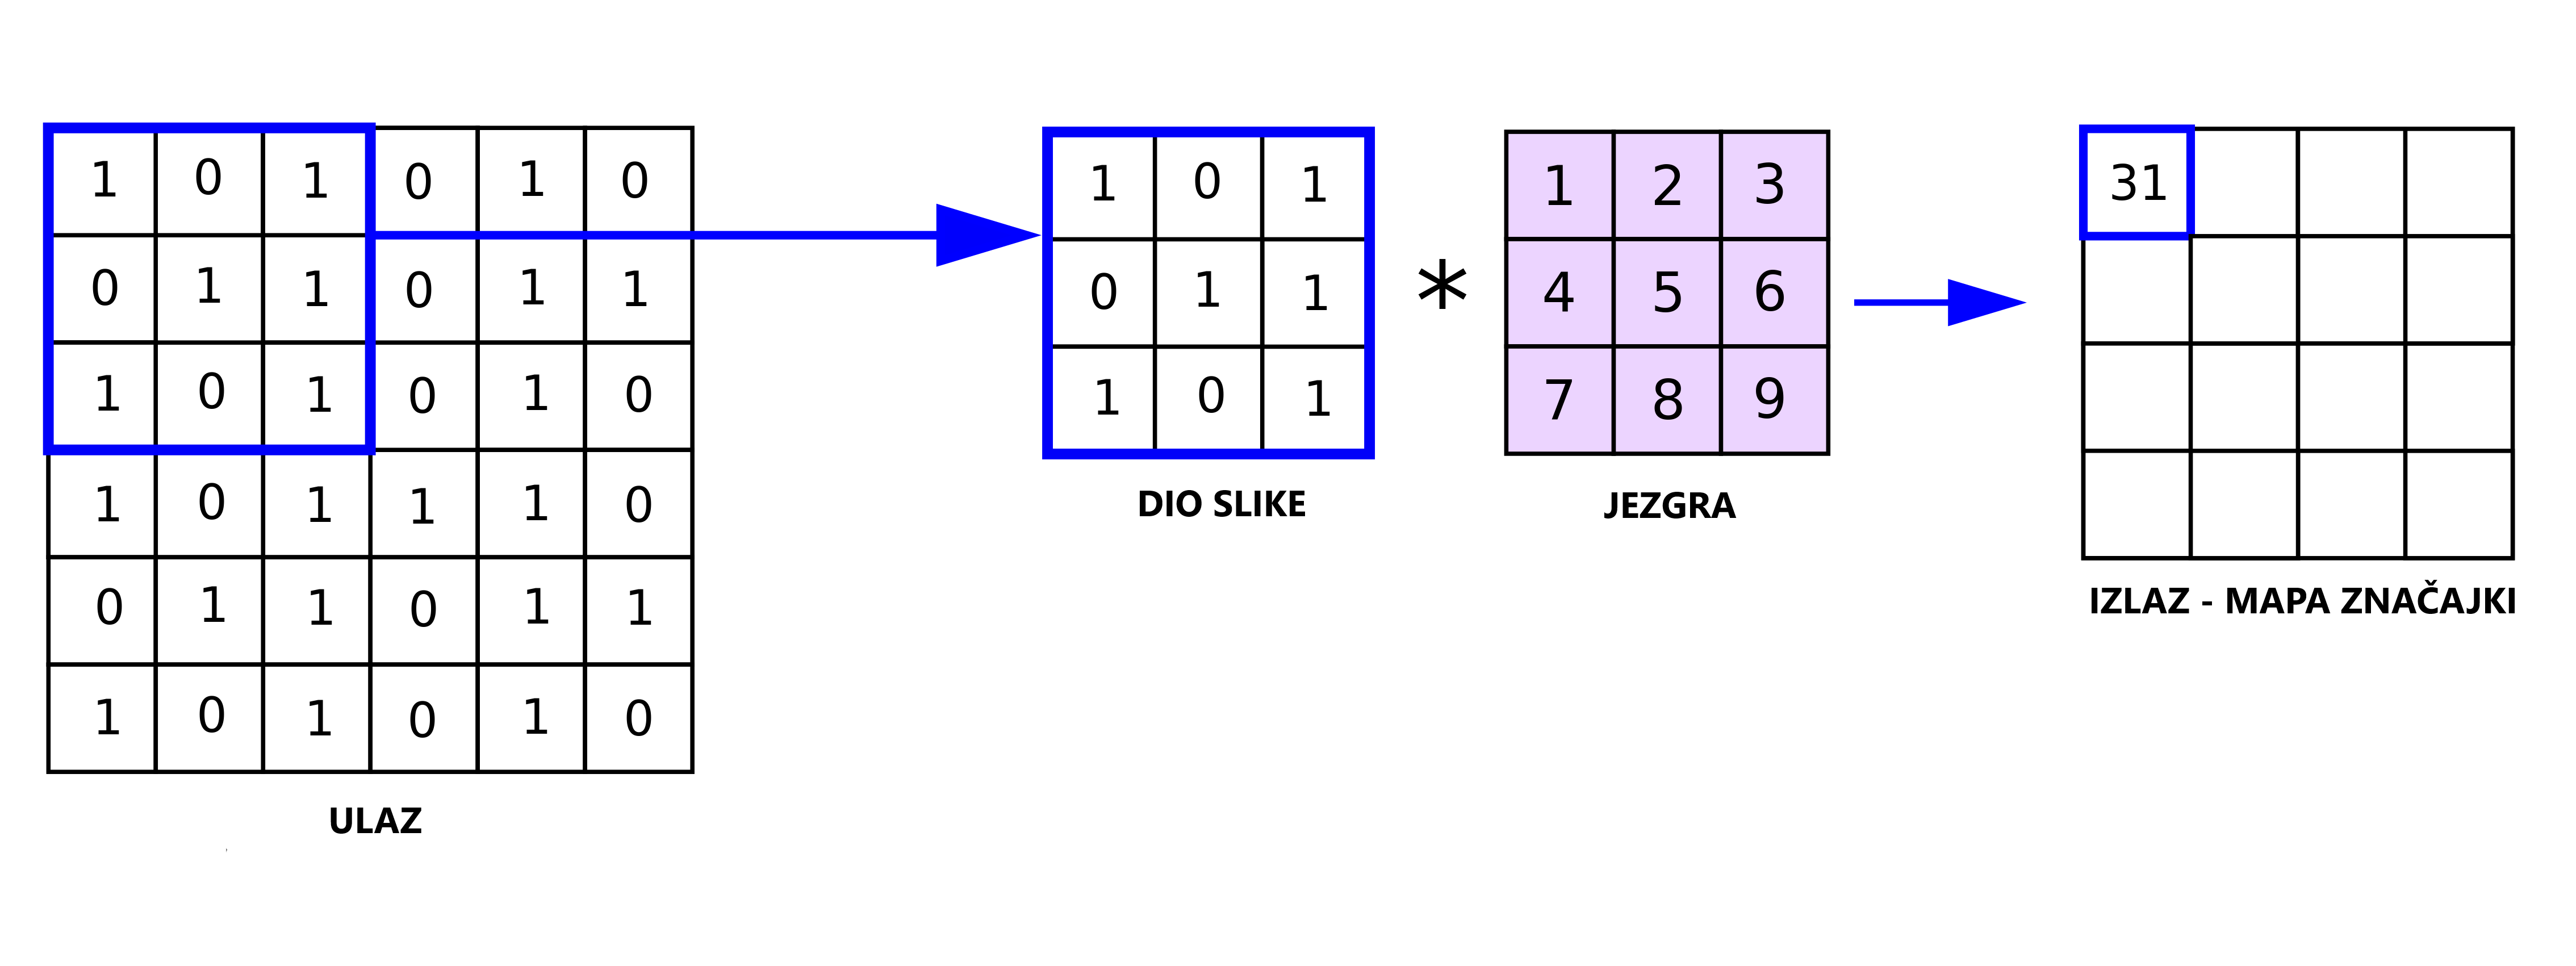
\includegraphics[width=15cm]{slike/kernelCNN.png}
\caption{Operacija konvolucije u CNN-u \citep{CNNAnnReynolds}}
\label{fig:fer-logo}
\end{figure}
\textbf{}


\noindent Nakon svakog konvolucijskog sloja, nad dobivenom mapom značajki primjenjuje se neka aktivacijska funkcija, koja je nužno nelinearna. Ako se sjetimo poglavlja 3.1.3, znamo da je nelinearnost aktivacijske funkcije bitna kako bi mreža bila u stanju modelirati složenije pojave. Najčešće korištena aktivacijska funkcija u konvolucijskim mrežama je \textbf{ReLU} \engl{Rectified Linear Units}. U svojoj osnovi, ReLU je vrlo jednostavna funkcija:

$$ReLU(x) =\begin{cases}0 & x  \leq  0\\x & x > 0\end{cases} $$

\noindent Glavne prednosti ReLU nad ostalim nelinearnim aktivacijskim funkcijama, poput sigmoide ili tangensa hiperbolnog su 

\begin{enumerate}
  \item Vrlo lagan izračun u odnosu na alternative - samo treba odrediti je li x veći ili manji od 0
  \item Derivacija ReLU je uvijek 0 ili 1. Ovo je izuzetno korisno u rješavanju problema tzv. nestajućeg gradijenta \engl{vanishing gradient}, koji je karakterističan za neke funkcije poput sigmoide. Problem se javlja zbog činjenice da derivacije sigmoidalnih funkcija teže 0 kada x -> $\infty$. ReLU, čija je derivacija uvijek 0 ili 1 nema takav problem, čime se omogućuje algoritmu propagacije pogreške da nastavi čak i za velike ulazne vrijednosti.  \citep{baeldungReLU}
\end{enumerate}

\noindent \textbf{Sloj sažimanja} \engl{pooling layer} ima kao cilj smanjiti dimenziju mape značajki, te time smanjiti broj parametara i resursne zahtjeve modela. Također ima za ulogu učiniti model manje osjetljivim na manje promjene u ulazima, time poboljšavajući generalizaciju modela. Veličinu dijela mape značajki nad kojim se provodi sažimanje određuje \textbf{dimenzija sažimanja}, dok veličinu pomaka, kao i kod konvolucijskog sloja, određuje \textbf{korak}. Naravno, veličina koraka u ovom sloju nije ni na koji način povezana s veličinom koraka u konvolucijskom sloju. Sam postupak sažimanja je vrlo sličan postupku u konvolucijskom sloju - idemo po dijelovima mape značajki, te za svaki dio računamo sažetak koristeći funkciju sažimanja. Sažetak zatim mapiramo na izlaz ovog sloja.

Razlikujemo dvije vrste sažimanja - \textbf{sažimanje po maksimalnoj vrijednosti} \engl{max pooling} te \textbf{sažimanje po prosječnoj vrijednost} \engl{average pooling}. Sažimanje po maksimalnoj vrijednosti za svaki dio ulaza (mape značajki) vraća njegovu maksimalnu vrijednost kao izlaz. Sažimanje po prosječnoj vrijednosti za svaki dio ulaza vraća njegovu prosječnu vrijednost. Između ova dva pristupa, preporučuje se korištenje sažimanja po maksimalnoj vrijednosti, jer uz smanjenje dimenzionalnosti, pridonosi i uklanjanju šuma iz ulaza. \cite{towardsDSCNN} \\

\begin{figure}[htb]
\centering
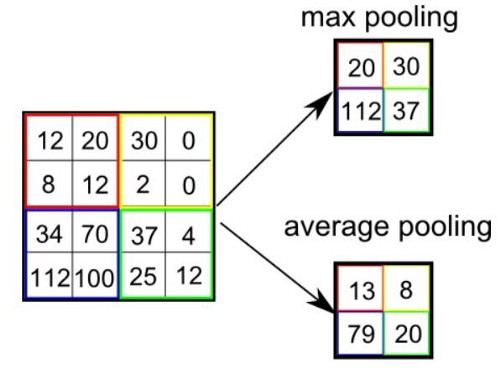
\includegraphics[height=6cm]{slike/poolingLayer.png}
\caption{Sloj sažimanja \citep{towardsDSCNN}}
\label{fig:fer-logo}
\end{figure}
\textbf{}

\noindent U nekim primjenama, primjerice klasifikacija slika, dodaje se i treći sloj, tzv. \textbf{potpuno povezani sloj} \engl{fully connected layer}. Ovaj sloj se nalazi pri kraju mreže, te na njega dolaze izlazi prethodna dva sloja, najčešće pretvoreni u jednodimenzionalni vektor. Ovaj dio konvolucijske mreže se zatim ponaša kao obična neuronska mreža.

\noindent Sve slojeve konvolucijske neuronske mreže možemo vidjeti na slici 3.6\\



\begin{figure}[htb]
\hspace{-2cm}
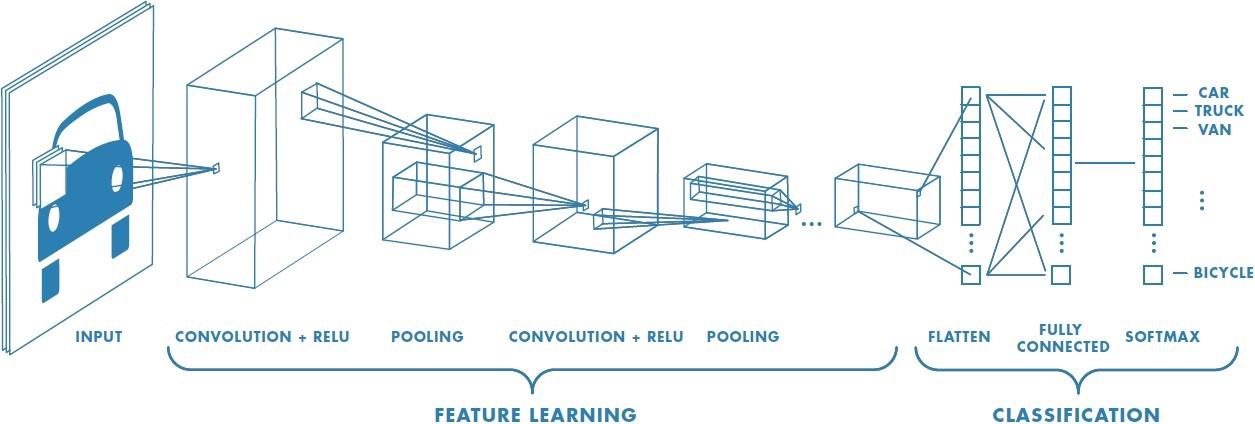
\includegraphics[width=17cm]{slike/CNNFull.jpeg}
\caption{Arhitektura konvolucijske neuronske mreže \citep{towardsDSCNN}}
\label{fig:fer-logo}
\end{figure}
\textbf{}


\section{Primjena u računalnom vidu i semantičkoj segmentaciji}
U ovom poglavlju ćemo pogledati kako se duboke neuronske mreže mogu iskoristiti za semantičku segmentaciju. Naglasak će biti na arhitekturama modificiranih konvolucijskih neuronskih mreža.

Generalni pristup semantičkoj segmentaciji korištenjem dubokih konvolucijskih modela možemo razdvojiti u dvije bitne komponente - \textbf{enkoder}, iza kojeg slijedi \textbf{dekoder}. Zadaća enkodera je obaviti klasifikaciju ulazne slike, na način opisan u poglavlju 3.2, no umjesto da rezultat klasifikacije koristeći potpuno povezani sloj dovedemo na izlaz mreže kao odluku o klasifikaciji slike, dovodimo ga na ulaz dekodera. Zatim je zadaća dekodera da naučenu klasifikaciju niže rezolucije projektira na izlaznu matricu, odnosno sliku, kako bi dobili gušću klasifikaciju, te u konačnici segmentacijsku mapu. Naravno, ovo je vrlo poopćen opis, te konkretni implementacijski detalji ovise o korištenoj arhitekturi.

U nastavku ćemo pogledati par istaknutih dubokih konvolucijskih modela koji, među ostalim, imaju primjenu u računalnom vidu i semantičkoj segmentaciji


\subsection{ResNet}
ResNet je, uz AlexNet, jedan od najpoznatijih dubokih modela u svijetu računalnog vida. Ova mreža je poznata po svojoj velikoj dubini (152 sloja), te uvođenju koncepta rezidualne jedinice.

ResNet kreće od ideje da, iako povećanje dubine mreže rezultira boljim performansama, također otežava treniranje. Ovo je najviše zbog pojave problema nestajućeg gradijenta (već spomenut u poglavlju 3.2.1), te slične pojave zvane eksplodirajući gradijent \engl{exploding gradient}. Oba ova problema postaju izraženija povećanjem dubine mreže.

Kako bi riješili ovaj problem, originalni autori uvode pojam \textbf{rezidualne jedinice} \engl{residual block}, prikazanog na slici 3.7 Na slici vidimo da se ulazni podaci, prilikom ulaska u neki od konvolucijskih slojeva, također nepromijenjeni šalju nekoliko slojeva dalje. Ovo je korisno zato što omogućava lakšu propagaciju gradijenta prilikom propagacije pogreške unazad. Konkretan primjer - ako jedan od konvolucijskih slojeva radi više štete nego koristi - recimo vodi do povećavanja funkcije pogreške umjesto smanjenja, koristeći ResNet arhitekturu praktički ga možemo ignorirati, jer imamo drugi put do ostatka mreže, stvoren grananjem rezidualne jedinice. Također, pošto je taj "alternativni" put ustvari put prema nepromijenjenom ulazu, ako odaberemo taj put efektivno smanjujemo dubinu mreže. Na ovaj način, dodatni slojevi mreže se koristi samo ukoliko pomaže u smanjenju funkcije gubitka. Ukoliko ne pomažu, mreža modificira težine na takav način da se prilikom dolaska do te rezidualne jedince uvijek odabere "zaobilazni" put, te na taj način efektivno smanji dubina mreže. U originalnom radu, \citep{resnetOriginal} ResNet arhitektura je korištena za problem klasifikacije slika, no manjim modifikacijama arhitekture te uvođenjem dekodera, primjenjiva je i za probleme semantičke segmentacije.

ResNet nije glavna tema ovog rada, stoga u dodatne implementacijske detalje neću ulaziti, no zainteresiranom čitatelju za daljnje istraživanje preporučujem originalni članak o ResNet arhitekturi \citep{resnetOriginal}, te članak \citep{resnetDecodingArhitecture}, koji na razumljiv i čitak način objašnjavaju ključne komponente arhitekture.

\begin{figure}[htb]
\centering
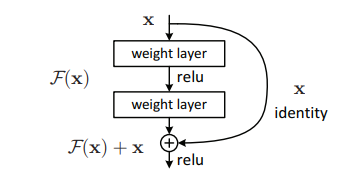
\includegraphics[width=13cm]{slike/resnet.png}
\caption{Rezidualna jedinica, ključna komponenta ResNet arhitekture \citep{resnetOriginal}}
\label{fig:fer-logo}
\end{figure}
\textbf{}\\


\subsection{U-net}
Osnovna motivacija nastanka U-net arhitekture je bila omogućiti dobre rezultate semantičke segmentacije uz relativno malenu količinu podataka. Razvijena je s ciljem segmentacije medicinskih slika, te je u tom području pokazala vrlo dobre rezultate. Formalno, ova arhitektura pripada u tzv. \textbf{potpuno konvolucijske mreže} \engl{fully convoluted neural networks, FCNN}, konvolucijske mreže koje se sastoje samo od konvolucijskih slojeva i slojeva sažimanja.

Najbolji način za razumijevanje arhitekture ove mreže je kroz skicu arhitekture, prikazanu na slici 3.8

\begin{figure}[htb]
\centering
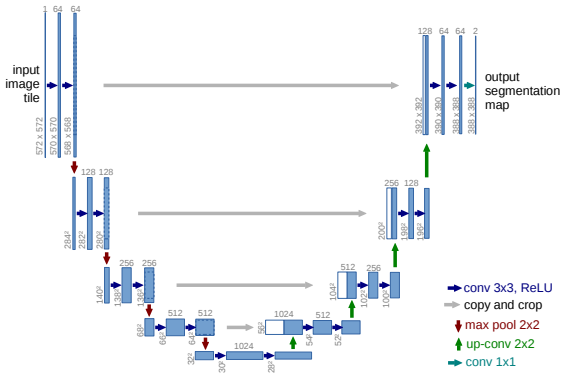
\includegraphics[width=13cm]{slike/unet.png}
\caption{U-net arhitektura. \citep{unetOriginal}}
\label{fig:fer-logo}
\end{figure}
\textbf{}

\noindent Na slici, svaki plavi kvadrat predstavlja višekanalnu mapu atributa. Broj na vrhu kvadrata predstavlja broj kanala u mapi, dok je sa strane dana i dimenzija mape. Strelicama različitih boja označene su operacije unutar mreže (legenda na slici).

Vidimo da se mreža sastoji od dva suprotna dijela - enkoderski dio, u kojem ulazna slika prolaskom kroz konvolucijske slojeve i slojeve sažimanja biva sve više i više poduzorkovana \engl{downsampling}. Ovime dobivamo mapu značajki malih dimenzija pomoću koje model može raspoznati veća grupiranja piksela iste klase na ulaznoj slici. Međutim, kako je dobivena slika vrlo malih dimenzija, potrebno je provesti proces naduzorkovanja \engl{upsampling}, u kojem se, koristeći proces "obrnute konvolucije", slici povećava rezolucija. Kako ne bi došlo do prekomjernog gubitka informacija prilikom povećanja rezolucije, koristan je velik broj kanala koji svaka mapa atributa ima. U zadnjem sloju dekoderskog dijela završavamo s mapom atributa jednake rezolucije kao i ulazna slika. U tom sloju se dodatno provodi 1x1 konvolucija, koja kao cilj ima mapirati dobivenu mapu atributa u odgovarajući broj klasa.

Prilikom treniranja, autori predlažu korištenje procesa augmentacije podataka, kako bi se poboljšalo svojstvo generalizacije mreže i smanjila količina potrebnih podataka.


\subsection{Deeplab}
Deeplab je zajednički naziv za obitelj dubokih neuronskih mreža razvijanih od strane Googlea. Trenutno postoje 4 verzije Deeplab arhitekture, od kojih je najnoviji DeeplabV3+ iz 2018.

U svojoj osnovi, Deeplab je modifikacija ResNet arhitekture, gdje se za proces enkodiranja, odnosno poduzorkovanja koristi manji broj slojeva sažimanja u kombinaciji sa \textbf{ dilatiranom konvolucijom} \engl{atrous convolution}. Ova vrsta konvolucija omogućava obrade većeg dijela slike manjom jezgrom, odnosno polje slike nad kojim se primjenjuje konvolucija ima veće dimenzije od same jezgre. Nedostajući podaci se nadopunjuju nulama. Parametar koji određuje stupanj dilatacije konvolucije naziva se \textbf{stopa dilatacije}. Primjerice, jezgra dimenzija 3x3 sa stopom dilatacije 2 pokriva područje veličine 5x5 originalne slike. Ovakav pristup omogućava pokrivanje većeg dijela slike koristeći konvoluciju s manjim brojem parametara. U Deeplab arhitekturi ovo svojstvo iskorištavamo tako da originalnu sliku poduzorkujemo manji broj puta nego što je to slučaj u ostalim arhitekturama. Umjesto toga, "povećavamo" efektivnu veličinu filtera koristeći dilatirane konvolucije umjesto običnih, te zatim te filtere primjenjujemo nad poduzorkovanim slikama. Primijetimo, dvije su glavne prednosti ovog pristupa: \citep{towardsDeeplab}

\begin{enumerate}
  \item Smanjenjenjem potrebnog broja operacija poduzorkovanja, ubrzavamo rad modela
  \item Kako konvolucije sad provodimo na slikama većih dimenzija (zbog manjeg broja poduzorkovanja), ovo nam omogućava da primjenom filtera izvučemo više značajki iz njih nego što je slučaj sa slikama manjih dimenzija, te samim time dobijemo točniju mapu značajki
\end{enumerate}
 
 DeeplabV2 i DeeplabV3 uvode još nekoliko modifikacija, poput piramidalnog dilatiranog sažimanja i oštrije detekcije rubova na slikama.


\chapter{Generativni modeli}

U ovom poglavlju pogledat ćemo jedan drugačiji pristup učenju. Tehnike i arhitekture s kojima smo se do sada bavili mogli bismo okarakterizirati kao \textbf{diskriminativne} - cilj nam je bio povezati uzorke skupa za učenje sa odgovarajućim oznakama (klasa slike, oznake piksela itd.) S druge strane, \textbf{generativni} pristup nastoji što točnije naučiti distribuciju podataka za učenje, kako bi na osnovu njih mogao generirati nove podatke iz te distribucije. Primijetimo da rezultati ova dva pristupa mogu biti identični, no način na koji dolazimo do rezultata je fundamentalno različit. Za određene primjene, generativni modeli su se u praksi pokazali kao puno bolji izbor od diskriminativnih.

Malo formalnije, ako imamo zadan skup ulaznih podataka X te set očekivanih izlaza Y, diskriminativni modeli pokušavaju naučiti uvjetnu vjerojatnost $P(Y|X)$. Dakle, diskriminativne modele ne zanima koja je vjerojatnost pojave takvog para, nego samo što će biti s izlazom Y ako se na ulazu pojavi X. S druge strane, generativni modeli uče vjerojatnost $P(X,Y)$, odnosno mogu naučiti koja je vjerojatnost pojave konkretnog ulaza X i ulaza Y u isto vrijeme. Dakle oni uče i koja je vjerojatnost pojave određene kombinacije ulaza i izlaza

Konačno, pogledajmo razliku u pristupima diskriminativnog i generativnog modela na jednom konkretnom primjeru, prikazan na slici 3.9. Primjer je preuzet iz \citep{generativeGoogle}

\begin{figure}[htb]
\centering
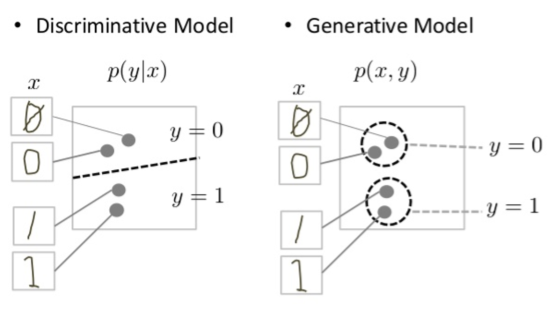
\includegraphics[width=12cm]{slike/generative_v_discriminative.png}
\caption{Diskriminativni vs generativni pristup \citep{generativeGoogle}}
\label{fig:fer-logo}
\end{figure}
\textbf{}

\noindent Razlika je objašnjenja u razlici pristupu problemu klasifikacije slika rukom napisanih znamenki, vrlo čestog primjera u području računalnog vida. Diskriminativni model nastoji odrediti razliku između dvije prikazane klase, 0 i 1, povlačenjem linije u prostoru svih podataka. Ta linija dijeli prostor na dva dijela - prostor u kojem su podaci koje je potrebno klasificirati kao 0, te prostor u koji pripadaju podaci koje je potrebno klasificirati kao 1. Ako model dobro "pogodi" poziciju te linije, može uspješno klasificirati dane ulaze u jednu od te dvije klase, bez da ikad mora naučiti koja je točna pozicija konkretnih ulaza u tom prostoru. S druge strane, generativni model nastoji naučiti točne pozicije konkretnih ulaza u prostoru podataka, dakle moraju naučiti na koji način su podaci \textbf{distribuirani} u prostoru podataka. Očito je da je to znatno složeniji pristup u odnosu na diskriminativni model, no to mu također omogućuje generiranje novih podataka iz dane distribucije.\\

\noindent U nastavku ćemo detaljnije pogledati primjere danas vrlo popularne obitelji arhitektura generativnih modela, zasnivanih na GAN arhitekturi.



\section{GAN}
\textbf{Generativna suparnička mreža} \engl{generative adversarial network, GAN} je naziv za arhitekturu dubokih generativnih modela prvi put predloženu od strane Goodfellowa i dr. u njihovom poznatom radu \citep{GoodfellowGAN}.

Autori predlažu arhitekturu koja se sastoji od 2 suparničke mreže - \textbf{generatora}, G i \textbf{diskriminatora} D. G je generativni model čija je zadaća što točnije naučiti distribuciju ulaznih podataka te generirati nove ("lažne") primjerke iz te distribucije. D je diskriminativni model čija je zadaća za dani ulaz odrediti vjerojatnost dolazi li iz skupa ulaznih (originalnih, pravih) podataka ili se radi o "lažnom" primjerku ulaza koji je G generirao. G se trenira tako da nastoji maksimizirati vjerojatnost da D napravi pogrešku, dok D treniramo tako da njegove procjene budu što točnije. Ovakav pristup odgovara igri \textbf{minimaks} sa 2 igrača, G i D, u kojoj svaki igrač nastoji maksimizirati vjerojatnost svoje pobjede i minimizirati vjerojatnost pobjede protivnika (provjeri je li ovo dobra interpretacija minimaxa!). Kako želimo da generator generira što točnije uzorke iz ciljne distribucije, konačni cilj ove igre je situacija u kojoj je G savršeno naučio ulaznu distribuciju i može generirati podatke praktički jednake onima iz ulazne distrucije, dok D za svaki ulaz daje vjerojatnost 0.5 jer ne može razaznati radi li se o originalnom ili "lažnom" podatku.

Kako bismo formalno definirali funkciju cilja ove arhitekture, uvedimo sljedeću nomenklaturu. Neka nam $x$ predstavlja određeni ulazni podatak (primjerice 2D sliku). Sa $D(x)$ ćemo označiti diskriminatorsku mrežu koja za dani ulaz $x$ vraća skalar - vjerojatnost da $x$ dolazi iz podataka za treniranje, a ne iz generatora. Ukoliko $x$ dolazi iz podataka za treniranje, očekujemo da će izlaz $D(x)$ biti velik, dok za slučaj kad je $x$ izlaz generatora očekujemo da će $D(x)$ biti malen. $D(x)$ se dakle ponaša kao običan binarni klasifikator. Nadalje, sa $z$ označimo slučajni vektor iz normalne distribucije. $G(z)$ će onda biti generatorska funkcija koja mapira $z$ na prostor ulaznih podataka. Kao što smo već rekli, cilj $G(z)$ je što točnije naučiti distribuciju ulaznih podataka kako bi to mapiranje bilo što točnije. Iz navedenog slijedi da sa $D(G(z))$ možemo označiti vjerojatnost s kojom je  $D(x)$ siguran da izlaz generatora $G(z)$ dolazi iz originalnog skupa podataka. Konačno, funkciju cilja ove arhitekture možemo definirati kao: 

\NewEnviron{myequation}{%
    \begin{equation}
    \scalebox{1}{$\BODY$}
    \end{equation}
    }

\begin{myequation}%
\bm{\mathop{min}\limits_{G}\mathop{max}\limits_{d}V(D,G) = \mathbb{E}_{x \sim p_{data}(x) } [logD(x)] + \mathbb{E}_{x \sim p_{z}(z)}[log(1-D(G(z)))]
}  %
\end{myequation}

\noindent gdje $\mathbb{E}_{x \sim p_{data}(x) }$ predstavlja očekivanu vrijednost nad svim pravim ulazima, a $\mathbb{E}_{x \sim p_{z}(z)}$ očekivanu vrijednost nad svim lažnim (generiranim) ulazima. D nastoji maksimizirati $logD(x)$, vjerojatnost da će uspješno klasificirati ulazne podatke. G nastoji minimizirati vjerojatnost $(log(1-D(G(z)))$, odnosno da će D ispravno klasificirati njegove izlaze kao lažne.

Autori također navode da u ranim fazama treniranja, dok generator još nije dobro naučio ciljnu distribuciju ulaza, D može raspoznavati prave od lažnih ulaza s vrlo visokom točnosti, što može dovesti do zasićenja $log(1 − D(G(z)))$, odnosno do toga da GAN "zapne" prilikom treniranja. Kao alternativu možemo trenirati G da maksimizira $log D(G(z))$ umjesto da minimizira $log(1 − D(G(z)))$. Ovo u osnovi predstavlja istu ideju, samo što ovaj rezultira puno strmijim gradijentima u ranoj fazi treniranja.\\


\noindent Treniranje GAN-a je zahtijevnije od treniranja ostalih dubokih modela iz dva razloga: 

\begin{enumerate}[label=(\alph*)]
\item Moramo uspješno trenirati 2 mreže: generator i diskriminator
\item Konvergenciju GAN-a je teško definirati, a time i otkriti
\end{enumerate}

Stoga GAN-ove obično treniramo na tako da prvo fiksiramo parametre generatora i treniramo diskriminator jednu ili više epoha. Ovo je potrebno jer u suštini diskriminator treniramo da prepozna mane u generatoru; kad bi istovremeno mijenjali diskriminator i generator, to bi bio gotovo nemoguć problem. Slično u sljedećem koraku: fiksiramo parametre diskriminatora te treniramo generator. Također, bitno je treniranje zaustaviti na vrijeme, obično kada diskriminator više ne može razlikovati prave ulaze od lažnih. Ako nastavimo trenirati nakon te točke, generator se trenira na pogrešnim povratnim informacijama od diskriminatora, te može doći do pogoršanja njegovih performansi. \\

\noindent Puni algoritam za treniranje dajem u nastavku.

\begin{algorithm}
  \caption{Algoritam treniranja generativnih suparničkih mreža}
  \begin{algorithmic}
      \For{broj iteracija}
        \For{k koraka}
            \begin{itemize}
              \item Uzmi m slučajnih uzoraka šuma ${(z^{(1)}...z^{(m)})}$
              \item Uzmi m ulaznih primjera ${(x^{(1)}...x^{(m)})}$ iz skupa ulaznih podataka
              \item Ažuriraj diskriminator penjući se njegovim stohastičkim gradijentom: 
              $$\nabla_{ \Theta _{d}} \cdot\frac{1}{m}  \sum\limits_{i=1}^m [log D(x^{(i)} + log(1-D(G(z^{(i)})))]$$
            \end{itemize}
        \EndFor
            \begin{itemize}
              \item Uzmi m slučajnih uzoraka šuma ${(z^{(1)}...z^{(m)})}$
              \item Ažuriraj generator spuštajući se njegovim stohastičkim gradijentom: 
              $$\nabla_{ \Theta _{g}} \cdot\frac{1}{m}  \sum\limits_{i=1}^m log(1-d(G(z^{(i)})))$$
            \end{itemize}
        \EndFor
 \end{algorithmic}
\end{algorithm}

\section{cGAN}
\textbf{Uvjetne generativne suparničke mreže } \engl{conditional generative adversarial networks, cGAN}, prvi put predstavljene u \citep{cGAN}, su nadogradnja na postojeću GAN arhitekturu nastale s ciljem usmjeravanja izlaza GAN-a. U običnoj GAN arhitekturi, ne možemo kontrolirati izlaz mreže, jer se izlaz bazira na slučajnom vektoru koji GAN mapira u odgovarajući izlaz.  cGAN rješava ovaj problem tako da priliom treniranja provodi uvjetovanje diskriminatora i generatora pomoću dodatne informacije, $y$. Ta dodatna informacija može biti bilo što, poput oznaka klasa, segmentacijskih mapa itd. Na taj način generator nauči da prilikom generiranja izlaza mora uzeti u obzir informaciju $y$. Jednom kada smo dovršili treniranje i želimo pokrenuti naš model u produkciji, za dobivanje željenog izlaza, primjerice segmentacijske mape dane slike, dovoljno je da kao ulaz u model damo sliku čiju segmentacijsku mapu želimo dobiti. Ta segmentacijska mapa predstavlja dodatnu informaciju $y$ uz pomoć koje cGAN generira izlaz - traženu segmentacijsku mapu dane slike.\\

\noindent Modificirana funkcija cilja cGAN-a je:

\begin{myequation}%
\bm{\mathop{min}\limits_{G}\mathop{max}\limits_{d}V(D,G) = \mathbb{E}_{x \sim p_{data}(x) } [logD(x|y)] + \mathbb{E}_{x \sim p_{z}(z)}[log(1-D(G(z|y)))]
}  %
\end{myequation}

\noindent Jedna poznata primjena cGAN modela je pix2pix arhitektura, koja služi za pretvorbu jedne vrste slika u drugu (npr. možemo naučiti mrežu da mapira slike konja na slike zebri).\\

\begin{figure}[htb]
\centering
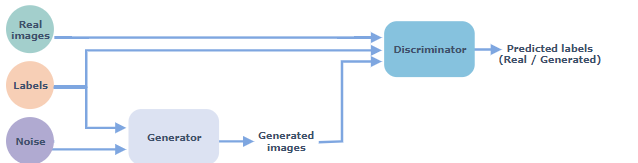
\includegraphics[width=14cm]{slike/cGAN.png}
\caption{Arhitektura cGAN mreže \citep{cGANImage}}
\label{fig:fer-logo}
\end{figure}
\textbf{}


\section{DCGAN}

Još ću se vrlo kratko osvrnuit na DCGAN arhitekturu \citep{dcgan}, modifikaciju GAN arhitekture posebno prilagođene za rad sa slikama. \textbf{Duboke konvolucije generativne suparničke mreže} \engl{deep convolutional adversarial generative networks, DCGAN} nadograđuju klasični GAN model uvodeći sljedeće izmjene:
\begin{itemize}
    \item {\large •} Slojeve sažimanja u diskriminatoru mijenja s konvolucijom s koracima \engl{strided convolution}, dok slojeve sažimanja u generatoru mijenja s konvolucijom s djelomičnim koracima \engl{ fractional-strided convolution}. Ovo omogućava mreži da sama nauči provoditi poduzorkovanje
    \item {\large •} Koristi \textit{batch} normalizaciju u generatoru i diskriminatoru
    \item {\large •} Uklanja potpuno povezane slojeve u dubljim arhitekturama
    \item {\large •} Koristi ReLU aktivacijsku funkciju u svim slojevima, osim u izlaznoj gdje koristi tangens hiperbolni
    \item {\large •} Koristi \textit{LeakyReLU} kao aktivacijsku funkciju u svim slojevima diskriminatora
\end{itemize}

\noindent Ove promjene poboljšavaju učenje, te u konačnici daju bolje rezultate u odnosu na klasični GAN. Također, autori su nakon treniranja mreže uspješno izdvojili diskriminatorski dio mreže te ga (samostalno) koristili kao klasifikator.


\section{cycleGAN}
Glavna motivacija za uvođenje arhitekture \textbf{cikličnih generativnih suparničkih mreža} \engl{cycle generative adversarial networks, cycleGAN} je problem prevođenja slika iz domene A u domenu B. Primjerice, želimo naučiti mrežu da za danu sliku livade u proljeće generira sliku iste livade ali recimo zimi. Ili na osnovu poznatog umjetničkog djela, primjerice Van Goghove \textit{Zvjezdane noći}, dobiti sliku koja izgleda kao fotografija krajolika na osnovu kojeg je djelo naslikano. Tradicionalni pristupi ovakvom problemu zahtijevaju velik broj povezanih parova slika iz domene A i domene B, odnosno za ulaznu sliku iz domene A model zahtijeva \textbf{istu} tu sliku, samo iz domene B. Konkretno na našem primjeru prevođenja slika livada u proljeće u slike, postojeći modeli zahtijevaju da im kao ulaz damo puno slika livada u proljeće, ali i u zimu. Očito je kako je u određenim situacijama vrlo nezgodno, pa čak i nemoguće doći do takvih parova (kako doći do fotografije krajolika koji je Van Gogh gledao kad je slikao \textit{Zvjezdanu noć}?)

Arhitektura cycleGAN, prvi put opisana u \citep{cycleGANOriginal}, rješava navedeni problem. U klasičnom (c)GAN pristupu, generator bi naučio mapiranje $G: X \longrightarrow Y$, gdje je X početna, a Y ciljna domena. U kombinaciji s diskriminatorom koji bi učio razliku između $y$ (originalnih ulaza) i $ \hat{y}$ (generiranih ulaza), G bi u idealnom slučaju savršeno naučio distribuciju od $Y$, te bi generirane slike bilo nemoguće raspoznati od originalnih slika. Međutim, ovo uvijek ne garantira da će originalni $x$ i generirani $y$ biti povezani na smislen način, jer postoji beskonačno mnogo mapiranja $G:X \longrightarrow Y$ koji će rezultirati savršenom distribucijom $y$. Također, kod ovakvog pristupa pojavljuje se \textit{mode collapse} problem, gdje se svi ulazni $x$ mapiraju na isti $y$, te učenje stagnira. Postoje određena rješenja ovih problema (evidentno iz postojanja pix2pix cGAN arhitekture spomenute u 4.2), no autori za rješavanje ovih problema predlažu da bi treniranje modela trebalo biti \textit{ciklički konzistentno}, odnosno da model paralelno uz učenje mapiranja $G:X \longrightarrow Y$, uči i inverzno mapiranje $F:Y \longrightarrow X$, odnosno G i F moraju biti inverzne funkcije, te ujedno i bijekcije. Tu praksi znači da ćemo u mreži imati dva generatora i dva diskriminatora. Prvi generator, G, uči mapiranje $G:X \longrightarrow Y$. Prvi diskriminator, $D_{y}$, uči razlikovati originalne slike iz skupa $X$ i slike iz $X$ koje generira G. Drugi generator, F, uči obrnuto mapiranje, $F:Y \longrightarrow X$, a drugi diskriminator, $D_{x}$, kako razlikovati originalne slike iz $Y$, te slike koje generira F. Slika 4.3 prikazuje navedenu arhitekturu.\\

\begin{figure}[htb]
\centering
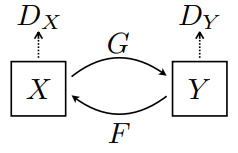
\includegraphics[width=8cm]{slike/cycleGAN1.png}
\caption{Generatori i diskriminatori cycleGAN arhitekture \citep{cycleGANOriginal}}
\label{fig:fer-logo}
\end{figure}
\textbf{}


\noindent Kako bi uspješno trenirali ovu mrežu, uvodimo nekoliko novih funkcija gubitka. Za generator G i pripadajući mu diskriminator $D_{y}$ izražavamo cilj kao:

\begin{myequation}%
\bm{\mathcal{L}_{GAN}(G,D_{y}, X, Y) = \mathbb{E}_{y \sim p_{data}(y) } [logD_{Y}(y))] + \mathbb{E}_{x \sim p_{data}(x)}[log(1-D_{Y}(G(x))]}  %
\end{myequation}

Kao i kod klasičnog GAN-a, G nastoji minimizirati ovu funkciju, dok ju D nastoji maksimizirati. Na ekvivalentan način definiramo i cilj za F i $D_{x}$:

\begin{myequation}%
\bm{\mathcal{L}_{GAN}(F,D_{x}, X, Y) = \mathbb{E}_{x \sim p_{data}(x) } [logD_{X}(x))] + \mathbb{E}_{y \sim p_{data}(y)}[log(1-D_{X}(F(y))]
}  %
\end{myequation}

Konačno, uvodimo pojam \textbf{ciklične funkcije gubitka} \engl{cycle loss}, kako bi osigurali da mapiranja G i F budu \textbf{ciklički konzistentna}. Odnosno da za svaku ulaznu sliku $x$, prolaskom kroz cijeli krug (ciklus) naše mreže, kao izlaz generatora F ponovno trebamo dobiti sliku $x$. Odnosno, želimo postići $x \longrightarrow G(x) \longrightarrow F(G(x)) = x$. Ovu relaciju zovemo \textbf{unaprijedna ciklična konzistentnost}. Također želimo postići i obrnuto, odnosno za svaku sliku iz domene $Y$, treba vrijediti $y \longrightarrow F(y) \longrightarrow G(F(y)) = y$. Model potičemo da nauči ovakvo ponašanje uvođenjem cikličke funkcije gubitka: 

\begin{myequation}%
\bm{\mathcal{L}(G,F) = \mathbb{E}_{x \sim p_{data}(x)}[||F(G(x)) -x||_{1}] + \mathbb{E}_{y \sim p_{data}(y)}[||G(F(y)) - y||_{1}]}  %
\end{myequation}

Ukupnu funkciju gubitka dobivamo zbrajanjem navedenih funkcija:

\begin{myequation}%
\bm{\mathcal{L} (G,F,D_{X},D_{Y}) = \mathcal{L}_{GAN}(G,D_{Y},X,Y) + \mathcal{L}_{GAN}(F,D_{x}, Y, X) + \lambda\mathcal{L}_{cyc}(G,F)
}  %
\end{myequation}


\noindent Na slici 4.4 vidimo neke od brojnih mogućih primjena cycleGAN arhitekture.

\begin{figure}[htb]
\hspace{-2cm}
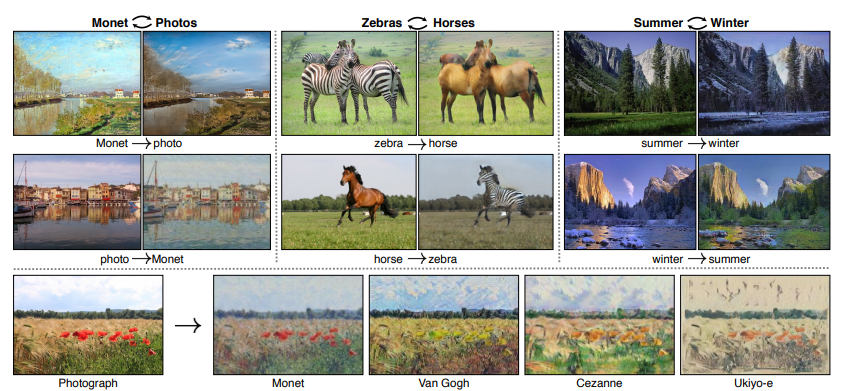
\includegraphics[width=18cm]{slike/cycleGAN2.png}
\caption{Primjene cycleGAN arhitekture \citep{cycleGANOriginal}}
\label{fig:fer-logo}
\end{figure}
\textbf{}

\chapter{Korištenje cycleGAN arhitekture za semantičku segmentaciju ortopanograma}

\section{Opis problema}

Jedan od najčešće korištenih, pa i najkorisnijih dijagnostičkih alata u području stomatologije su zasigurno rendgenske panoramske snimke čeljusti. Relativno su jednostavne za provođenje, a stomatologu daju velik broj informacija o stanju pacijenta. Međutim, u određenim situacijama, poput prisustva šuma u ortopanogramu, ili većeg broja umjetnih zubi/implanata čak i najboljem stomatologu može biti zahtjevno odrediti točnu poziciju svakog od zuba u čeljusti. Stoga bi programsko rješenje koje bi omogućilo automatsko označavanje svakog zuba u ortopanogramu zasigurno bilo korisno, te bi se, uz primjenu kao pomoćni alat stomatolozima, moglo iskoristiti kao početna točka daljnjim nadogradnjama, poput automatske detekcije bolesti zuba ili slično. Stoga u ovom poglavlju predlažem rješenje za semantičku segmentaciju stomatoloških panoramskih rendgenskih snimaka, temeljnog na cycleGAN arhitekturi.\\

\noindent Kao podatke za treniranje predloženog modela na raspolaganju sam imao dvije vrste ortopanograma: 376 ortopanograma te njihovih pripadajućih segmentacijskih mapa (označenih ručno), te 3950 neoznačenih ortopanograma, odnosno ortopanograma bez pripadajuće segmentacijske mape. Upravo ovakva distribucija podataka, gdje na raspolaganju imamo relativno malen broj označenih slika ali relativno velik broj neoznačenih, je bila glavna motivacija za uvođenje cycleGAN arhitekture. Ta arhitektura bi u teoriji, uz sve označene slike, trebala moći iskoristiti i neoznačene slike prilikom treniranja kako bi poboljšala generalizaciju. 


\begin{figure}%
    \subfloat[Ortopanogram]{{\hspace*{-1cm}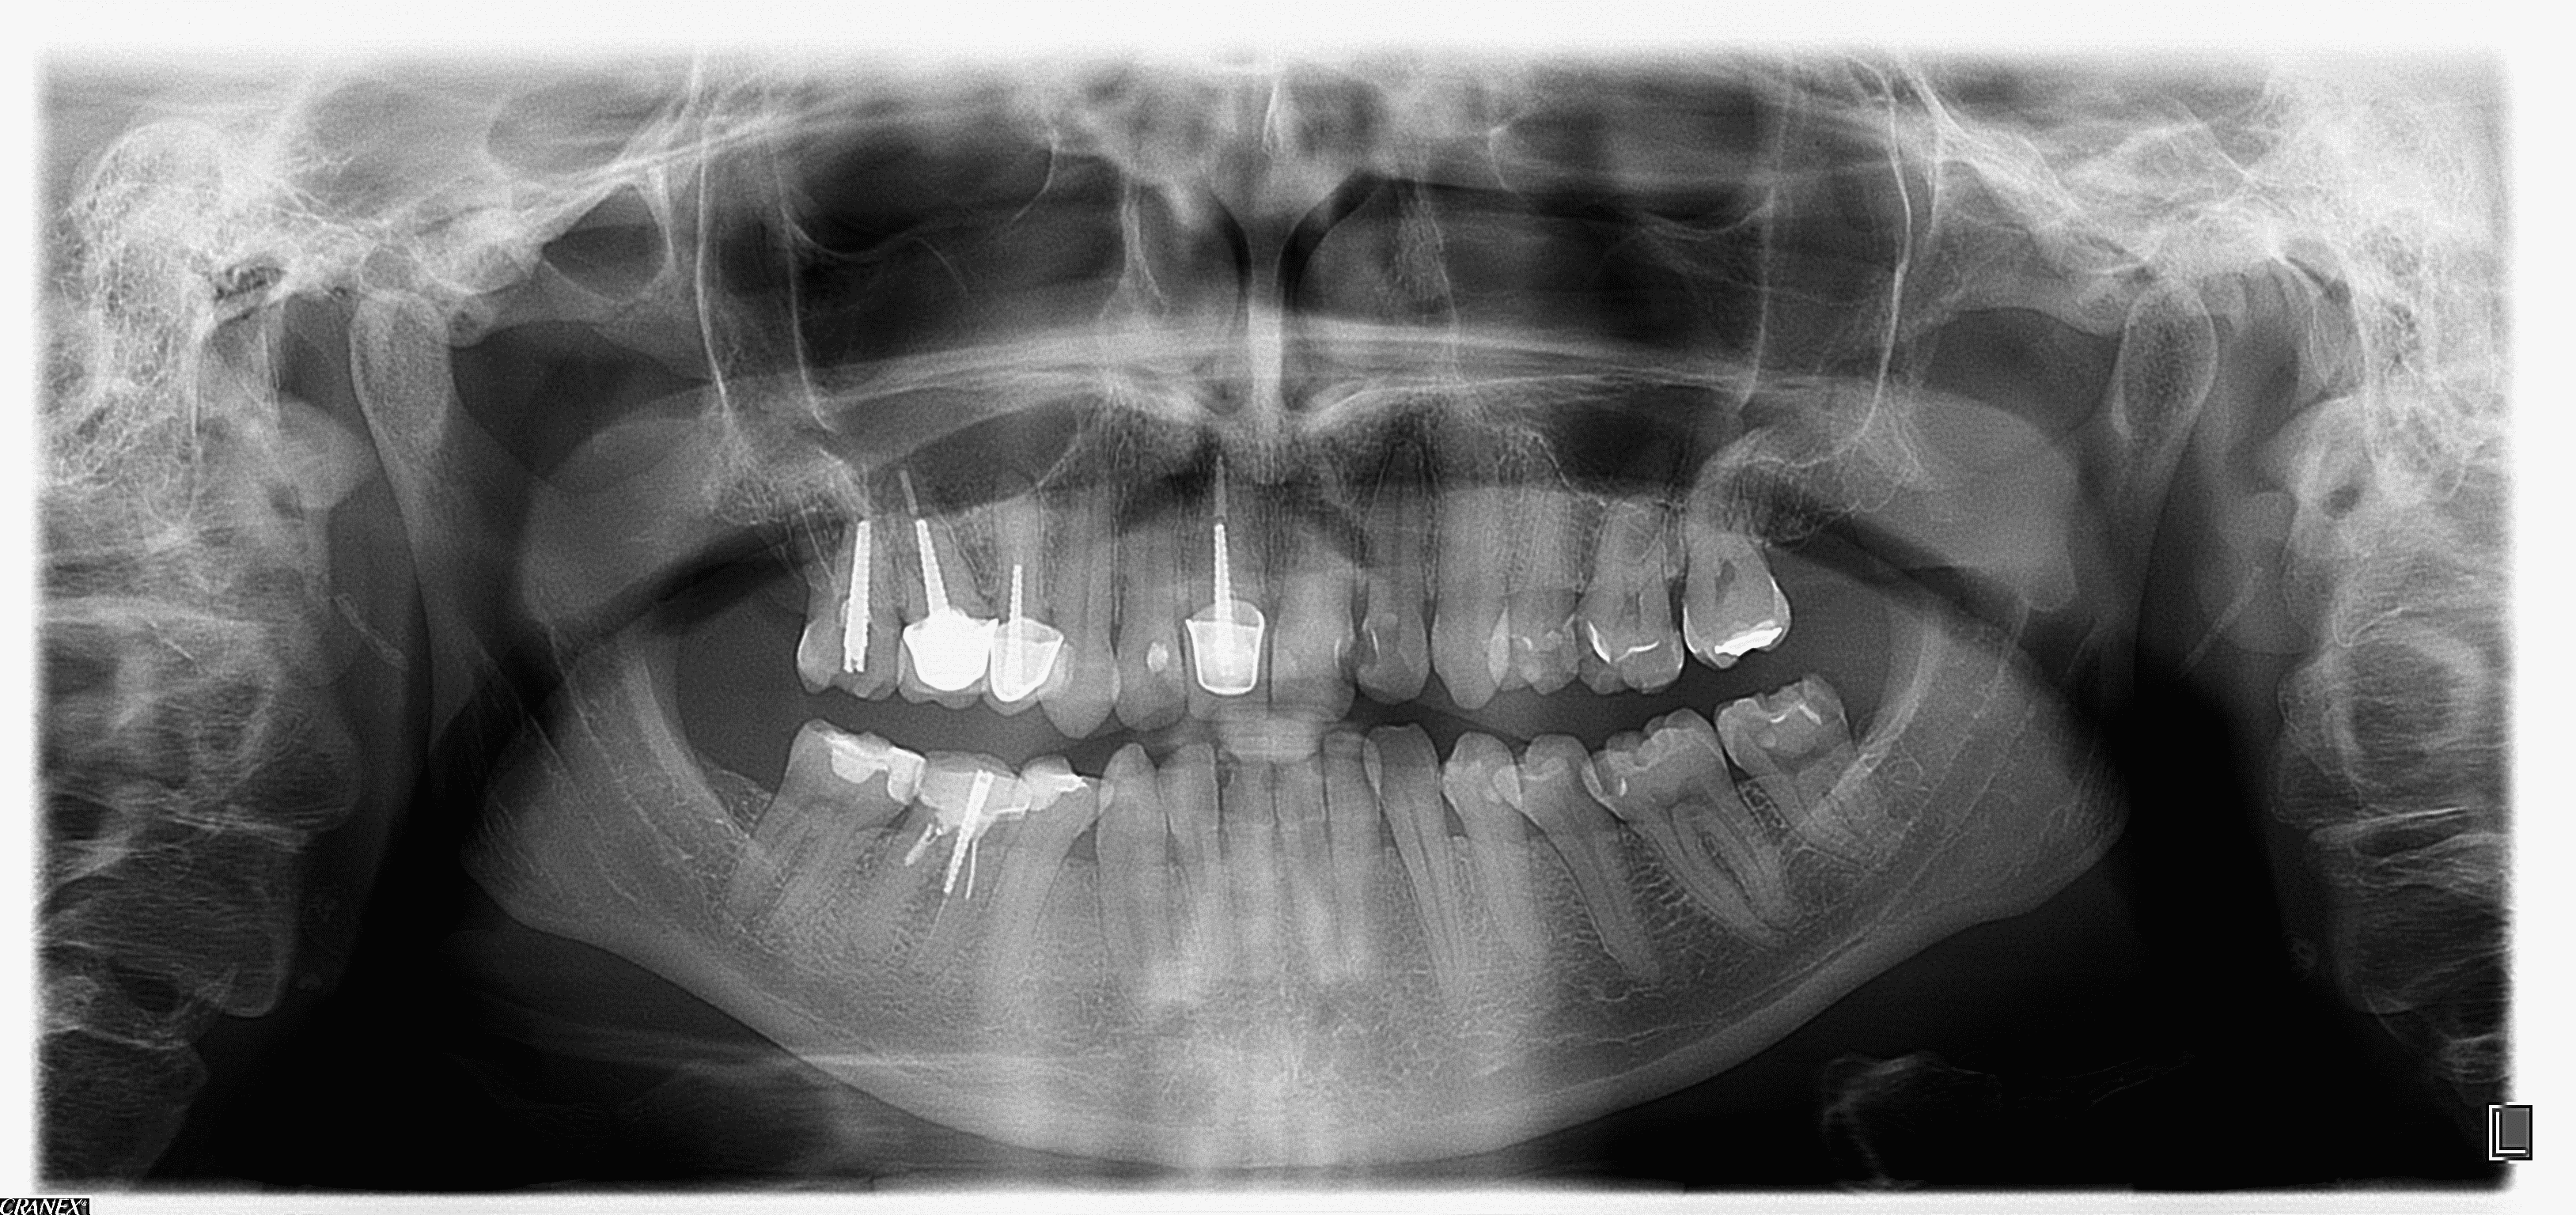
\includegraphics[width=16cm]{slike/ortopanogramPrimjer.png} }}%
    \qquad
    \subfloat[Ortopanogram + segmentacijska mapa]{{\hspace*{-1cm}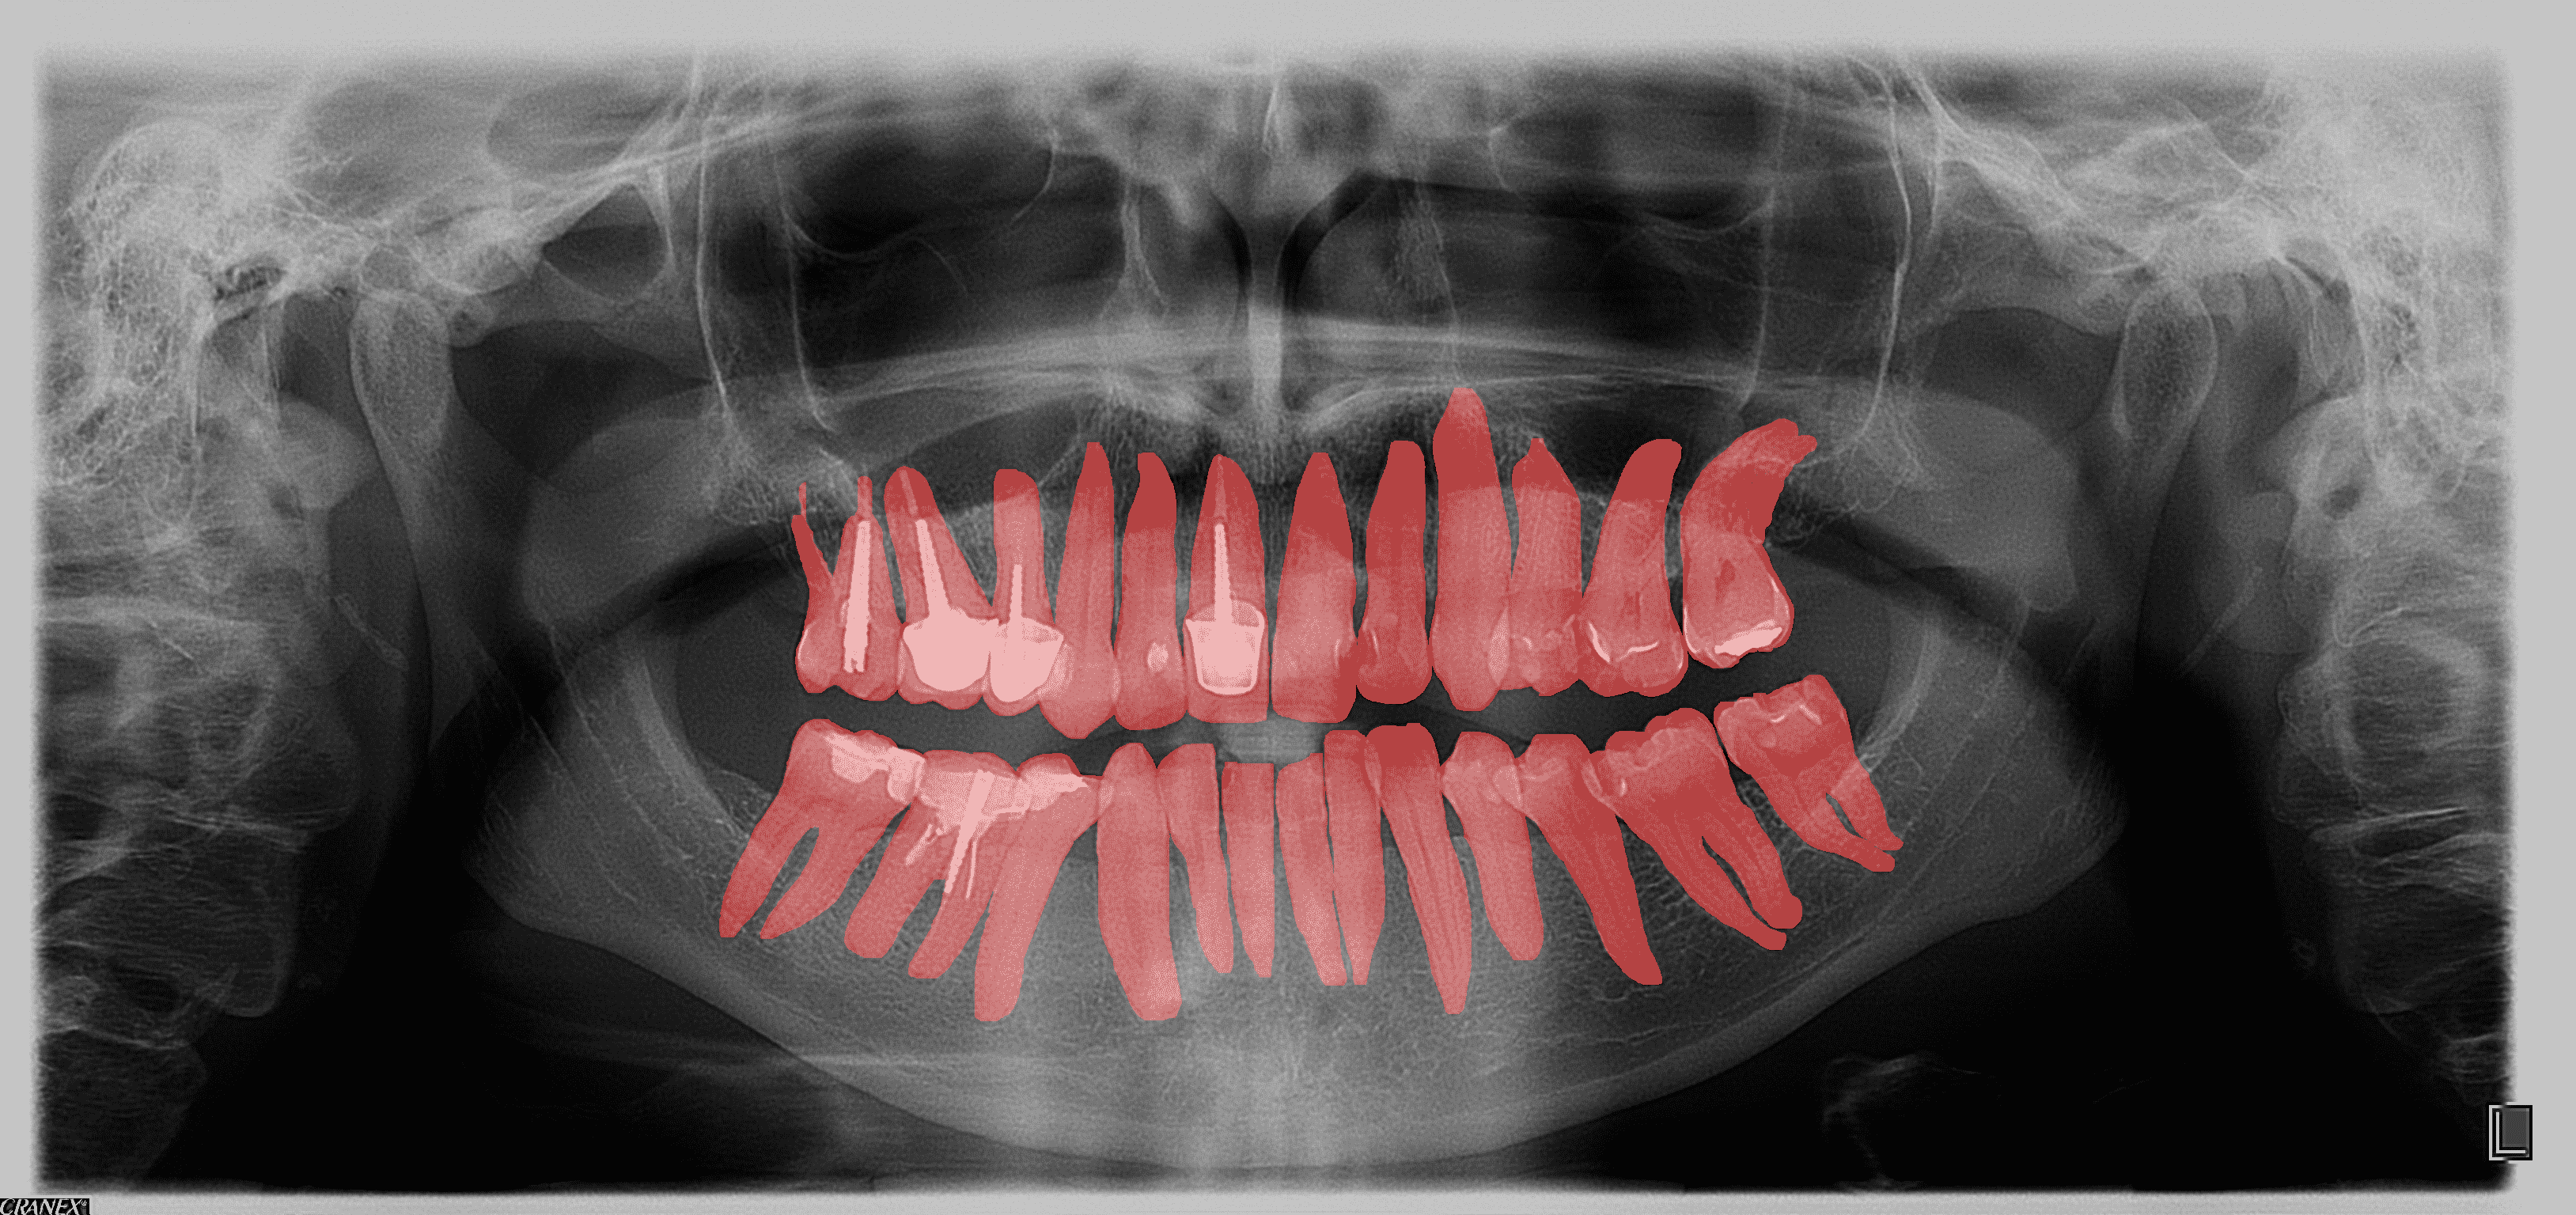
\includegraphics[width=16cm]{slike/ortopanogramPrimjerSegmentacija.png} }}%
    \caption{Ortopanogram i njegova segmentacijska mapa}%
    \label{fig:example}%
\end{figure}



\section{Opis predloženog rješenja}
Korišteno je rješenje prvi put predloženo u \citep{cycleGANSegmentation}. U tom radu autori predlažu iskorištavanje mogućnosti cycleGAN-a za učenje bidirekcijskog mapiranja korištenjem neuparenih slika iz domene A i domene B za polunadziranu semantičku segmentaciju. Navode da korištenjem svojstva cikličke konzistentnosti cycleGAN-a (opisanog u 4.4) model može naučiti bidirekcijsko mapiranje između \textbf{neoznačenih} slika i segmentacijskih mapa. Ovime dodajemo određeni nenadzirani regularizacijski efekt koji poboljšava treniranje, te također imamo način za iskoristiti i neoznačene slike u modelu, do kojih je često puno lakše doći nego do označenih. Baš zato što, uz klasične parove (slika, segmentacijska mapa) koristimo i dodatne neoznačene slike, koje nemaju svoje segmentacijske mape model vrši oblik \textbf{polunadziranog} \engl{semisupervised} učenja. Autori su proveli testiranje predloženog modela na tri skupa podataka (PASCAL VOC 2012, Cityscapes, ACDC), te zaključili da model postiže 2-4\% bolje rezultate u odnosu na odgovarajući potpuno nadzirani model.

U nastavku ću detaljnije opisati arhitekturu korištenog rješenja, kao i modifikacije potrebe za rad s ortopanogramima.
\subsection{Arhitektura rješenja}

Predložena arhitektura rješenja nešto je drugačija od običnog cycleGAN-a. 
Kao i kod običnog cycleGAN modela, predloženi model ima 2 generatora i 2 diskriminatora.Zadaća prvog generatora, kojeg ćemo označiti sa \bm{$G_{IS}$} (od engl. \textit{image to segmentation}), je mapirati slike (ortopanograme) na njihove odgovarajuće segmentacijske mape. Prvi diskriminator, \bm{$D_{S}$}, nastoji razlikovati te generirane segmentacijske mape od originalnih. Drugi generator, \bm{$G_{SI}$} \engl{segmentation to image}, uči kako mapirati segmentacijsku mapu s odgovarajućom slikom tj. ortopanogramom. Ovaj generator se koristi samo za poboljšanje treniranja. Konačno, drugi diskriminator \bm{$D_{I}$} kao ulaz prima sliku ortopanograma te nastoji odrediti radi li se o stvarnoj ili generiranoj slici. Kako bi se osigurala ciklička konzistentnost, generatori se treniraju tako da kad segmentacijsku mapu koju je generirao $G_{IS}$ predamo u $G_{SI}$ kao izlaz dobijemo originalnu sliku ortopanograma. I obrnuto, kad generatoru $G_{IS}$ predamo sliku koju je generirao $G_{SI}$, kao izlaz dobiti originalnu segmentacijsku mapu koju je $G_{SI}$ primio kao ulaz.

No, nije sve tako jednostavno. Uz dodatak opisanim generatorima i diskriminatorima, model ima još dva para generatora, nazovimo ih $\hat{G}_{IS}$, $\hat{G}_{SI}$, te još jedan dodatni diskriminator, $\hat{D}_{I}$. Zanimljivo je da se ovi dodatni generatori i diskriminatori ne spominju u originalnom radu, već su ih autori naknadno dodali u \textbf{službeni} kod modela, priložen radu, uz još nekoliko izmjena. Jedino objašnjenje koje je dano je da se radi o "daljnjim poboljšanjima". Ove 3 mreže se u kodu isključivo koriste na mjestima gdje bi se u običnom cycleGAN-u računala tzv. ciklična pogreška slika. Koriste se na način da diskriminator $\hat{D}_{I}$ odlučuje dolazi li rekonstruirana slika iz ciklusa $\hat{G}_{IS}$, $\hat{G}_{SI}$, ili iz ciklusa 
$G_{IS}$, $G_{SI}$. Iako nisam sasvim siguran zašto su autori odlučili uvesti ove izmjene, u praksi se pokazalo da značajno pridonose uspješnosti modela (mIoU 0.5 za originalni model vs mIoU 0.65 za modificirani model, 33 klase). Iz tog razloga odlučio sam koristiti modificiranu arhitekturu umjesto one predložene u samom radu.\\

\noindent Kako bi formalnije definirali predloženu arhitekturu, kao i korištene funkcije gubitka, uvedimo sljedeću nomenklaturu: sa \bm{$\mathcal{X_{L}}$} označimo skup označenih slika (dakle ortopanograma koji u skupu segmentacijskih maski imaju svoj par), sa \bm{$\mathcal{Y_{L}}$} skup svih originalnih segmentacijskih maski \engl{ground truth}, te sa \bm{$\mathcal{X_{U}}$} skup svih neoznačenih slika ortopanograma (dakle ortopanograma koji nemaju svoj par u skupu segmentacijskih maski). 

Uvodimo prvu funkciju gubitka, \bm{$L^{S}_{gen}$}. Radi se o nadziranoj funkciji pogreške za segmentaciju, čija je zadaća naučiti $G_{IS}$ da, na osnovu predane slike ortopanograma generira odgovarajuću segmentacijsku mapu. Funkciju definiramo kao:

\begin{myequation}%
\bm{L^{S}_{gen}(G_{IS}) = \mathbb{E}_{x,y \sim \mathcal{X_{L}}, \mathcal{Y_{L}}}[\mathcal{H}(y,G_{IS}(x)]}  %
\end{myequation}

\noindent gdje $\mathcal{H}$ predstavlja \textbf{unakrsnu entropiju} \engl{cross-entropy} po pikselima:

\begin{myequation}%
\bm{\mathcal{H}(y,  \hat{y}) =  \sum\limits_{j=1}^N   \sum\limits_{k=1}^K y_{j,k}log\hat{y}_{j,k}  }  %
\end{myequation}

\noindent U danoj jednadžbi za $\mathcal{H}$, $y_{j,k}$ predstavlja vjerojatnosti da piksel $j \; \epsilon \; (1, ..., N)$ originalne segmentacijske mape ima oznaku $k \; \epsilon \; (1, ..., K)$, gdje je K broj oznaka. Kako se radi originalnim oznakama, za $y_{j,k}$ ta vjerojatnost je uvijek 1 ili 0 - piksel ili ima tu oznaku ili nema. 
$\hat{y}_{j,k}$ predstavlja slične vjerojatnosti, samo za generiranu segmentacijsku mapu.\\

\noindent Za $G_{SI}$ koristimo L1 normu kao nadziranu funkciju gubitka, kako bi procijenili razliku između originalne označene slike, te slike koju $G_{SI}$ generira iz njene pripadajuće segmentacijske mape:

\begin{myequation}%
\bm{L^{I}_{gen}(G_{SI}) = \mathbb{E}_{x,y \sim \mathcal{X_{L}}, \mathcal{Y_{L}}}[||G_{SI}(y) - x||_{1}]}  %
\end{myequation}

\noindent Prisjetimo se, L1 norma se računa kao apsolutna razlika između dobivenih i očekivanih vrijednosti.

\noindent Kako bi iskoristili neoznačene ortopanograme, uvodimo još dvije vrste funkcija gubitka: suparničke funkcije gubitka i funkcije gubitka za cikličku konzistentnost.

Ako je $D_{S}(y)$ predviđena vjerojatnost da segmentacijska mapa $y$ odgovara originalnoj segmentacijskoj mapi, suparničku funkciju gubitka za $D_{S}$ možemo definirati kao:

\begin{myequation}%
\bm{L^{S}_{disc}(G_{IS},D_{S}) = \mathbb{E}_{y \sim \mathcal{Y_{L}}}[MSE((D_{S}(y))] +
\mathbb{E}_{x' \sim \mathcal{x_{U}}}[MSE(( D_{s}(G_{IS}(x'))))]
}  %
\end{myequation}

Vidimo da se ustvari radi u funkciji srednje kvadratne greške \engl{mean squared error, MSE}. Funkcija se računa na osnovu uspjeha diskriminatora u razlikovanju pravih i lažnih segmentacijskih mapa. \\

\noindent Funkciju gubitka za drugi diskriminator, $D_{I}$, definiramo na ekvivalentan način:

\begin{myequation}%
\bm{L^{I}_{disc}(G_{SI},D_{S}) = \mathbb{E}_{y \sim \mathcal{Y_{L}}}[MSE(D_{S}(y))] + 
\mathbb{E}_{x' \sim \mathcal{x_{U}}}[MSE(( D_{s}(G_{IS}(x'))]
}  %
\end{myequation}

\noindent Prvu cikličku funkciju gubitka definiramo za segmentacijske mape. Kao što smo rekli, za svaki y (segmentacijsku mapu) očekujemo sljedeće: $G_{IS}(G_{SI}(y))  = y$. Ovakvo ponašanje možemo poticati koristeći sljedeću funkciju gubitka:


\begin{myequation}%
\bm{L_{cycle}^s(G_{IS}, G_{SI}) = \mathbb{E}_{{y \sim y_{\mathcal{L}}}}[\mathcal{H}(y, G_{IS}(G_{SI}(y)))]}  %
\end{myequation}

\noindent Koristimo unakrsnu entropiju jer su labele u segmentacijskim mapama kategorijske varijable. \\

\noindent Pogledajmo još uloge $\hat{G}_{IS}$ ,$\hat{G}_{SI}$ i $\hat{D}_{I}$. Prilikom treniranja generatora, $\hat{D}_{I}$ na ulazu prima rekonstruiranu sliku iz ciklusa $G_{SI}(G_{IS}(\mathcal{X_{U}}))$, te određuje  dolazi li rekonstruirana slika iz ciklusa $G_{SI}(G_{IS}(\mathcal{X_{U}}))$, ili iz ciklusa $\hat{G}_{SI}(\hat{G}_{IS}(\mathcal{X_{U}}))$. Na osnovu te odluke, koristeći MSE, računa se funkcija gubitka za $\hat{D}_{I}$. Tu funkciju gubitka možemo označiti sa $\bm{L_{D_{I}}^1}$.

Tijekom druge faze treniranja, kada treniramo diskriminatore a generatori su fiksirani, računamo funkciju gubitka $L_{D_{I}}^2$, kao:

\begin{myequation}%
\bm{L_{D_{I}}^2 = MSE(\hat{D_{i}}(\hat{G}_{SI}(\hat{G}_{IS}(x))),0) + MSE(\hat{D_{i}}({G}_{SI}({G}_{IS}(x))),1)}  %
\end{myequation}

\noindent Primijetimo, ova funkcija je slična $L_{D_{I}}^1$, samo što u nju ulazi i odluka o rekonstruiranoj slici iz ciklusa  $\hat{G}_{SI}(\hat{G}_{IS}(\mathcal{X_{U}}))$.\\

\noindent Konačno, ukupnu funkciju gubitka možemo napisati kao:

\begin{multline*}
L_{total} = \lambda_{1}L^{S}_{gen}(G_{IS}) + \lambda_{2}L^{I}_{gen}(G_{SI}) + \lambda_{3}L_{cycle}^s(G_{IS}, G_{SI}) -\\ \lambda_{4}L^{S}_{disc}(G_{IS},D_{S}) - \lambda_{5}L^{I}_{disc}(G_{SI},D_{S}) + \lambda_{6}L_{D_{I}}^1 - \lambda_{7}L_{D_{I}}^2
\end{multline*}

\noindent U praksi, treniramo generatore dok su parametri diskriminatora fiksirani, i obrnuto. \\

\noindent Kao što je već rečeno, generatori $G_{IS}$ i $G_{SI}$ zasnivani su na DeeplabV2 arhitekturi, dok su $\hat{G}_{IS}$ i $\hat{G}_{SI}$ zasnivani na ResNet arhitekturi. Korišteni su diskriminatori koji rade na razini piksela, odnosno diskriminator za svaki piksel donosi odluku je li lažan ili ne. Diskriminatori se sastoje od 3 konvolucijska sloja, nakon kojih dolazi \textit{Leaky ReLU} aktivacijska funkcija sa $\alpha = 0.2$.
\noindent Tijekom treniranja također je korišten Adam optimizator s parametrima $\beta_{1} = 0.5$ i $\beta_{2} = 0.999$. Stopa učenja postavljena je na 0.0002, s linearnim padom nakon svakih 100 epoha. U svim eksperimentima veličina grupe \engl{batch} je bila 2. Ukoliko u rezultatima modela nije drugačije navedeno, svi parametri $\lambda$ su jednaki 1.0.\\

\noindent Uz navedeni polunadzirani cycleGAN model, paralelno je treniran i nadzirani model (samo jedan generator, odnosno samostalna DeeplabV2 arhitektura), koji se bavi isključivo segmentacijom ortopanograma (dakle, nema veze s GAN-ovima). On je korišten kao usporedna točka za performanse cycleGAN modela.
\subsection{Programska implementacija}
Za programsku implementaciju korišten je programski jezik Python uz knjižnicu \textbf{\href{https://pytorch.org/}{Pytorch}}, a za praćenje treniranja modela koristan je bio alat \textbf{\href{https://www.tensorflow.org/tensorboard}{Tensorboard}}. Modifikacije koda većinom su uključivale prilagođavanje nove vrste podataka - ortopanograma i njihovih segmentacijskih mapa formatu u kojem ih je model očekivao. U tu svrhu napisan je novi dataloader (naziv za klasu u Pytorchu zaduženu za učitavanje podataka u model) za rad s ortopanogramima. Dodana je funkcionalnost za segmentaciju ortopanograma u 2 klase (pozadina + zubi), 3 klase (gornja zubi, donji zubi, pozadina) te 33 klase (32 zuba + pozadina). Također su bile potrebne manje modifikacije u glavnom dijelu koda, većinom kako bi se podržao rad s novim podacima, te modifikacije dijelova koda zaduženih za testiranje i validaciju. Model je treniran na serveru opremljenom s NVIDIA GeForce RTX 2080 grafičkom karticom, sa 11GB video memorije.
\section{Eksperimentalni rezultati} 

Za evaluaciju dobivenih rezultata korištena je mjera \textbf{srednjeg presjeka nad unijom} \engl{mean intersection over union, mIoU}. Ovo je jedna od najčešće korištenih metoda za evaluaciju segmentacijskih modela. Metoda se zasniva na računanju postotka područja nad kojim se generirana oznaka i stvarna oznaka podudaraju, podijeljeno s unijom njihovih ukupnih područja. U slučaju više od jedne klase, IoU se računa za svaku klasu zasebno, te se na kraju računa prosjek dobivenih veličina. Moguće vrijednosti IoU su [0,1], pri čemu bi vrijednost 1 imao model kod kojeg je svaki piksel generirane segmentacijske mape jednak svakom pikselu originalne segmentacijske mape. mIoU je samo prosječan IoU nad svim uzorcima za validaciju. Formalno, IoU definiramo kao

\begin{figure}[htb]
\centering
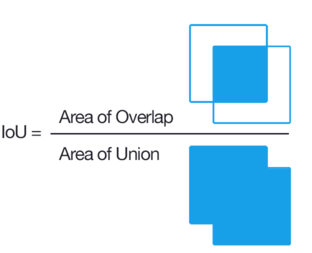
\includegraphics[width=8cm]{slike/miou.png}
\caption{Vizualizacija mIoU-a \citep{miou}}
\label{fig:fer-logo}
\end{figure}
\textbf{}


\noindent Dostupni označeni podaci za treniranje bili su podijeljeni u 3 kategorije: trening (250), validacija (61), testiranje (62). Ako se radilo o nenadziranom (cycleGAN) modelu, tada se u model još i učitavao slučajan podskup od 250 neoznačenih ortopanograma. Trenirani su modeli za segmentaciju 2, 3 i 33 klase. Svaki model je treniran prvo na na 400 epoha, s iznimkom modela s 3 klase, koji je treniran i na 200 epoha. Nakon treniranja tog modela na 200 epoha, zaključeno je da se bolji rezultati dobivaju s 400 epoha, pa su ostali modeli trenirani samo na 400 epoha. Prije ulaska u model, sve slike su postavljene na rezoluciju 200x400, zbog memorijskih ograničenja. Rezultati treniranja modela prikazani su u nastavku.\\

\begin{table}[htb]
\caption{Rezultati modela}
\label{tbl:konstante}
\centering
\begin{tabular}{llr} \hline
Model & Broj epoha & mIoU\\ \hline
Deeplab, 2 klase & 400 & 0.8729981767948044 \\
cycleGAN, 2 klase & 400 & 0.8735012386115315 \\
Deeplab, 3 klase & 200 & 0.8427474738296579 \\
cycleGAN, 3 klase & 200 & 0.8357329101641446 \\
Deeplab, 3 klase & 400 & 0.847020406648659 \\
cycleGAN, 3 klase & 400 & 0.8479922780975828\\
Deeplab, 33 klase & 400 & 0.7023904701665826\\
cycleGAN, 33 klase ($\lambda_{1} = 1.0$) & 400 & 0.650361416818396\\
cycleGAN, 33 klase ($\lambda_{1} = 1.25$) & 400 & 0.6810801346650556\\ \hline
\end{tabular}
\end{table}

\noindent Iz priložene tablice zaključujemo nekoliko stvari. Prva je da se povećanjem broja klasa mIoU smanjuje, no to nije ništa neočekivano. Vidimo da nadzirani (Deeplab) i polunadzirani (cycleGAN) model pri manjem broju klasa postižu gotovo identične rezultate - prilikom treniranja kroz 400 epoha cycleGAN je marginalno bolji, iako razlika je dovoljno mala da ju možemo zanemariti. Također vidimo da, prilikom treniranja sa 3 klase kroz 200 epoha nadzirani model je bio nešto bolji od polunadziranog. Međutim, kad smo broj epoha povećali na 400, polunadzirani model je uspio dostići, pa čak i prestići nadzirani model. Općenito sam primijetio da cycleGAN model sporije konvergira prema minimumu u odnosu na Deeplab model, pogotovo pri početku treniranja, te mogu zaključiti da je cycleGAN bolje trenirati kroz veći broj epoha u odnosu na nadzirane modele. \\ \\

\noindent Rezultati za 33 klase su nešto drugačiji. Vidimo da nadzirani model ima mIoU vrijednost za čak 0.05 bolju od polunadziranog modela, odnosno skoro 8\%. Ovakav rezultat nije u skladu s očekivanjima, jer su autori originalnog rada \citep{cycleGANSegmentation}, dobili bolje rezultate cycleGAN-a u odnosu na nadzirani model u svim slučajevima. Također, radili smo sa relativno malom količinom podataka (250 slika), te je bilo očekivano da će cycleGAN, uvođenjem dodatnih neoznačenih slika poboljšati treniranje. 

Smatram da razlog ovakvoj razlici između nadziranog i polunadziranog modela leži u činjenici da polunadzirani model jednostavno nije (dovoljno) dobro naučio generirati nove slike ortopanograma, što možemo vidjeti iz slika 5.9 te 5.10. Vidimo da je model dobro naučio generirati segmentacijske mape, no da nije bio toliko uspješan prilikom generiranja slika ortopanograma. Slike su mutne i pune šuma, što većinom nije bio slučaj u originalnom radu. Iako te slike jesu u većini slučaja bile dovoljne da bi model iz njih rekonstruirao segmentacijsku mapu ortopanograma, ta mapa se u većini slučajeva ipak djelomično razlikovala od originalne, što je zasigurno negativno utjecalo na treniranje modela. Smatram da je to dijelom zbog relativno malenog skupa podataka, a dijelom i zbog činjenice da su ulazne slike bile niske rezolucije, što odmaže treniranju modela. Također sam primijetio da je funkcija gubitka za diskriminator $D_{I}$ bila vrlo niska (<0.01), što ukazuje na to da je $D_{I}$ vrlo lako zaključivao da se radi o lažnim slikama, što ukazuje na njihovu lošu kvalitetu. Što se tiče funkcija gubitka diskriminatora, pokazivale su slično ponašanje kao i $D_{I}$.
Konačno, kako ukupna funkcija gubitka u cycleGAN modelu ovisi i o funkcijama gubitka zaduženim za generiranje slika, pretpostavljam da su upravo te funkcije gubitka zaustavljale ukupan model da ide prema nižem minimumu. Smatram da je to glavni razlog zašto je nadzirani model postigao bolje rezultate od nenadziranog. 

Djelomično kako bi testirao tu teoriju, a djelomično kako bi poboljšao rezultate modela, trenirao sam još jedan model - cycleGAN sa 33 klase, ali sa parametrom $\lambda_{1}$ povećanim sa 1.0 na 1.25. To je parametar koji određuje koliko funkcija gubitka generatora zaduženog za generiranje segmentacijskih mapa utječe na ukupnu funkciju gubitka. Pretpostavio sam da njegovo povećanje može potaknuti model da se u ukupnoj funkciji gubitka više fokusira na poboljšanje generiranja segmentacijskih mapa, te na taj način smanji utjecaj (loše) generiranih ortopanograma. Dobiveni rezultati potvrđuju tu pretpostavku - mIoU tog modela je za 0.03 uspješniji od mIoU-a istog modela sa $\lambda_{1}$ = 1.0, no i dalje je lošiji od nadziranog modela.\\


\noindent Kao ideju za neka buduća istraživanja, smatram da bi se bilo korisno fokusirati na poboljšanje generiranja neoznačenih slika u modelu, jer se to trenutno čini kao najslabiji dio modela. Korisno bi bilo i mijenjati ostale parametre modela (npr. $\lambda_{2}$, $\lambda_{3}$ itd.) da vidimo kako utječu na model. Također, kao i uvijek prilikom treniranja dubokih modela, rezultati modela bi sigurno bili bolji kada bi na raspolaganju imali više podataka. Bilo bi zanimljivo i pogledati kako rezolucija ulaznih slika utječe na performanse modela - očito je da bi rezultati modela bili bolji, no pitanje je u kojoj mjeri. Trenutno se pokazalo da je za problem segmentacije ortopanograma bolje koristiti neki klasičan konvolucijski model, poput Deeplaba, nego cycleGAN. Osim što se takav model pokazao bolji za segmentaciju većeg broja klasa, pokazuje gotovo identične performanse kao i cycleGAN kod nižeg broja klasa, a pošto puno brže konvergira, može ga se trenirati kroz manji broj epoha nego cycleGAN. Konačno, prilikom treniranja cycleGAN troši skoro 3x veću količinu memorije nego Deeplab (3GB vs 10.5GB), što ga čini prikladnijim i jednostavnijim za treniranje.\\


\noindent U nastavku prilažem slike koje su generirali odgovarajući modeli. U slučaju 2 klase, žutom bojom su označeni zubi, a crnom pozadina. Ako imamo 3 klase, žuto su donji zubi, a crveno gornji. Slično je u slučaju 33 klase, samo što je svaki donji zub označen svojom nijansom žute, a svaki gornji svojom nijansom crvene. \\


\begin{figure}
\begin{tabular}{cccc}
\hspace{-1.5cm}
{
\includegraphics[width = 8cm]{slike/rezultati/supervised2klase1.png}} &
{
\includegraphics[width = 8cm]{slike/rezultati/supervised2klase2.png}}\\
\hspace{-1.5cm}
{
\includegraphics[width = 8cm]{slike/rezultati/supervised2klase3.png}} &
{
\includegraphics[width = 8cm]{slike/rezultati/supervised2klase4.png}}\\
\end{tabular}
\caption{Neki od rezultata nadziranog modela za 2 klase}
\end{figure}

\begin{figure}
\begin{tabular}{cccc}
\hspace{-1.5cm}
{
\includegraphics[width = 8cm]{slike/rezultati/semisuper2klase1.png}} &
{
\includegraphics[width = 8cm]{slike/rezultati/semisuper2klase2.png}}\\
\hspace{-1.5cm}
{
\includegraphics[width = 8cm]{slike/rezultati/semisuper2klase3.png}} &
{
\includegraphics[width = 8cm]{slike/rezultati/semisuper2klase4.png}}\\
\end{tabular}
\caption{Neki od rezultata polunadziranog modela za 2 klase}
\end{figure}

\begin{figure}
\begin{tabular}{cccc}
\hspace{-1.5cm}
{
\includegraphics[width = 8cm]{slike/rezultati/super3klase1.png}} &
{
\includegraphics[width = 8cm]{slike/rezultati/super3klase2.png}}\\
\hspace{-1.5cm}
{
\includegraphics[width = 8cm]{slike/rezultati/super3klase3.png}} &
{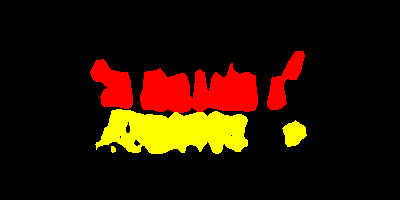
\includegraphics[width = 8cm]{slike/rezultati/super3klase4.png}}\\
\end{tabular}
\caption{Neki od rezultata nadziranog modela za 3 klase}
\end{figure}

\begin{figure}
\begin{tabular}{cccc}
\hspace{-1.5cm}
{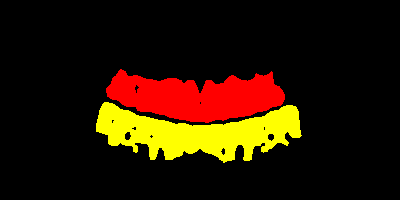
\includegraphics[width = 8cm]{slike/rezultati/semisuper3klase1.png}} &
{
\includegraphics[width = 8cm]{slike/rezultati/semisuper3klase2.png}}\\
\hspace{-1.5cm}
{
\includegraphics[width = 8cm]{slike/rezultati/semisuper3klase3.png}} &
{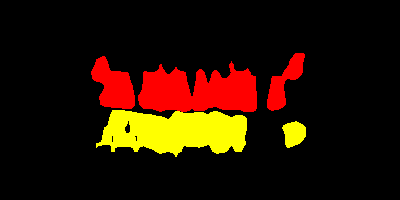
\includegraphics[width = 8cm]{slike/rezultati/semisuper3klase4.png}}\\
\end{tabular}
\caption{Neki od rezultata polunadziranog modela za 3 klase}
\end{figure}

\begin{figure}
\begin{tabular}{cccc}
\hspace{-1.5cm}
{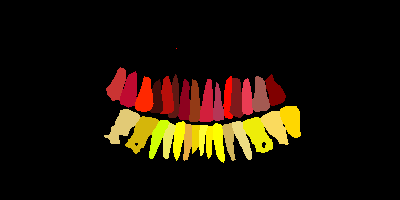
\includegraphics[width = 8cm]{slike/rezultati/super33klase1.png}} &
{
\includegraphics[width = 8cm]{slike/rezultati/super33klase2.png}}\\
\hspace{-1.5cm}
{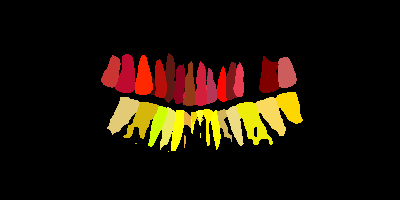
\includegraphics[width = 8cm]{slike/rezultati/super33klase3.png}} &
{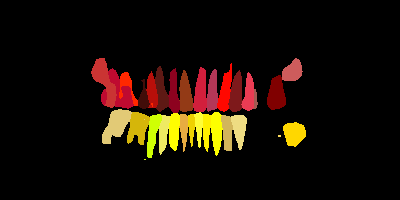
\includegraphics[width = 8cm]{slike/rezultati/super33klase4.png}}\\
\end{tabular}
\caption{Neki od rezultata nadziranog modela za 33 klase}
\end{figure}

\begin{figure}
\begin{tabular}{cccc}
\hspace{-1.5cm}
{
\includegraphics[width = 8cm]{slike/rezultati/semisuper33klase1.png}} &
{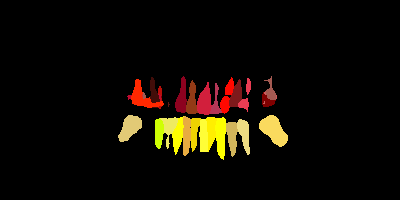
\includegraphics[width = 8cm]{slike/rezultati/semisuper33klase2.png}}\\
\hspace{-1.5cm}
{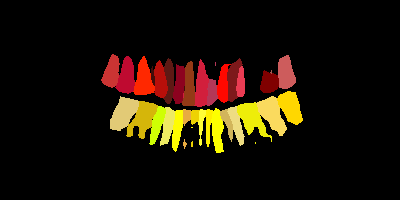
\includegraphics[width = 8cm]{slike/rezultati/semisuper33klase3.png}} &
{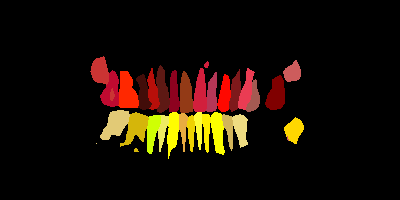
\includegraphics[width = 8cm]{slike/rezultati/semisuper33klase4.png}}\\
\end{tabular}
\caption{Neki od rezultata polunadziranog modela za 33 klase ($\lambda_{1} = 1.0$)}
\end{figure}

\begin{figure}
\begin{tabular}{cccc}
\hspace{-1.5cm}
\subcaptionbox{}{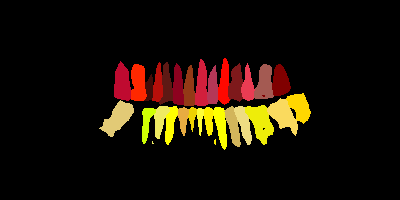
\includegraphics[width = 8cm]{slike/rezultati/train1.png}} &
\subcaptionbox{}{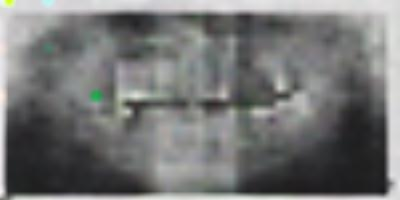
\includegraphics[width = 8cm]{slike/rezultati/train2.jpg}}\\
\hspace{-1.5cm}
\subcaptionbox{}{
\includegraphics[width = 8cm]{slike/rezultati/train3.jpg}} &
\subcaptionbox{}{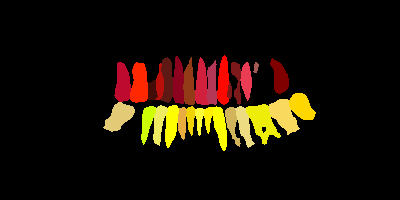
\includegraphics[width = 8cm]{slike/rezultati/train4.png}}\\
\end{tabular}
\caption{Prikaz svih generiranih slika tijekom jednog prolaska kroz cycleGAN mrežu, primjer. 1 Slika a) prikazuje prvi prolazak originalne slike kroz $G_{IS}$. Slika b) prikazuje sliku dobivenu prolaskom originalne segmentacijske mape kroz $G_{IS}$, dakle $G_{SI}(x)$. c) prikazuje sliku dobivenu prolaskom generirane segmentacijske mape kroz $G_{SI}$, dakle $G_{SI}(G_{IS}(x))$. d) prikazuje segmentacijsku mapu dobivenu prolaskom b) kroz $G_{IS}$.}
\end{figure}

\begin{figure}
\begin{tabular}{cccc}
\hspace{-1.5cm}
{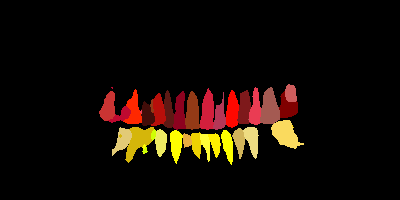
\includegraphics[width = 8cm]{slike/rezultati/train2a.png}} &
{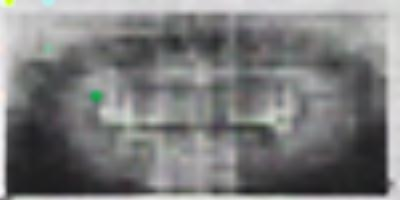
\includegraphics[width = 8cm]{slike/rezultati/train2b.jpg}}\\
\hspace{-1.5cm}
{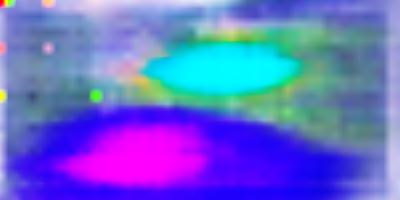
\includegraphics[width = 8cm]{slike/rezultati/train2c.jpg}} &
{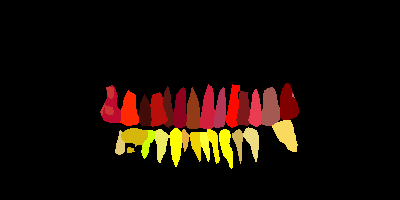
\includegraphics[width = 8cm]{slike/rezultati/train2d.png}}\\
\end{tabular}
\caption{Prikaz svih generiranih slika tijekom jednog prolaska kroz cycleGAN mrežu, primjer 2}
\end{figure}










\chapter{Zaključak}
Cilj ovog rada bio je pronaći odgovarajuće rješenje za problem semantičke segmentacije ortopanograma, u slučaju kad na raspolaganju imamo relativno malo označenih, a relativno puno neoznačenih slika. U tu svrhu ukratko su predstavljeni modeli dubokog učenja, s naglaskom na duboke konvolucijske modele, te je dano par primjera takvih arhitektura na konkretnom problemu semantičke segmentacije. Zatim je predstavljen koncept generativnih modela, te su predstavljene njihove prednosti nad klasičnim diskriminativnim modelima. Odabrana je jedna konkretna generatorska arhitektura, cycleGAN, iz razloga što, uz označene, može iskoristiti i neoznačene slike prilikom treniranja. Arhitektura je trenirana da raspozna 2, 3 i 33 klase u slici ortopanograma. Za treniranje je na raspolaganju bilo 250 označenih slika za treniranje, 62 slike za validaciju, 61 za testiranje i slučajan podskup od 250 slika od ukupno 3950 neoznačenih slika. Rezultati modela su pokazali da, iako je cycleGAN bio uspješan u problemu segmentacije, nije pokazao značajno bolje rezultate u odnosu na najnaprednije diskriminativne modele (Deeplab), te je u slučaju 33 klase čak pokazao lošije rezultate. Konačno, dano je par prijedloga za moguća daljna istraživanja.
\bibliography{literatura}
\bibliographystyle{fer}

\begin{sazetak}
Cilj ovog rada bio je pronaći i testirati odgovarajuću arhitekturu za problem semantičke segmentacije kada je prisutan manji broj označenih i veći broj neoznačenih primjera. Predstavljena je cycleGAN arhitektura, te je testirana na konkretnom problemu semantičke segmentacije ortopanograma. Arhitektura je izabrana iz razloga što može iskorisiti i neoznačene slike kao pomoć pri treniranju. Dobiveni rezultati su pokazali da cycleGAN arhitektura uspješno rješava navedeni problem, no da ipak zaostaje u usporedbi s najnaprednijim diskriminativnim modelima.

\kljucnerijeci{duboko učenje,konvolucijske neuronske mreže,semantička segmentacija, GAN, cycleGAN, ortopanogrami, medicinske snimke}
\end{sazetak}

% TODO: Navedite naslov na engleskom jeziku.
\engtitle{Segmentation of Stomatologic Panoramic X-ray Images}
\begin{abstract}
The goal of this work was to find and test an adequate deep learning architecture applicable to the problem of semantic segmentation, in the case when we at our disposal have a limited number of labeled images, but a relatively high amount of unlabeled images. cycleGAN, a type of generative model was  proposed as solution to the starting problem. It was chosen due to the fact that it can use unlabeled images as well as labeled to improve training performance. It was tested on the dataset of stomatologic X-ray images (orthopantomograms), and it was shown that while it successfully solves the given problem, it still falls behind most advanced discriminative models.

\keywords{deep learning,convolutional neural networks,semantic segmentation, GAN, cycleGAN, orthopantomograms, medical imaging}
\end{abstract}


\end{document}
